
%...........................................................
%
% Predicted spectra
%
%...........................................................

\section{Predicted $e$-like spectra}
\label{app:templates_elike}

In \cref{fig:joint_ereco_components} each flavor component 
of the neutrino and antineutrino mode $e$-like samples
is shown separately in order to compare the different shapes as a function of $E_{reco}$.
The NC spectrum distribution,
which is the largest component of the background,
is quite flat over all the energy range and is quite difficult to separate.
The $\nu_{\mu} \rightarrow \nu_e$ and $\bar{\nu}_{\mu} \rightarrow \bar{\nu}_e$ events
populate the same energy region, around 0.6 GeV, with a very similar shape.

\begin{figure*}[htb]
%\hspace{0.06\linewidth}
\center
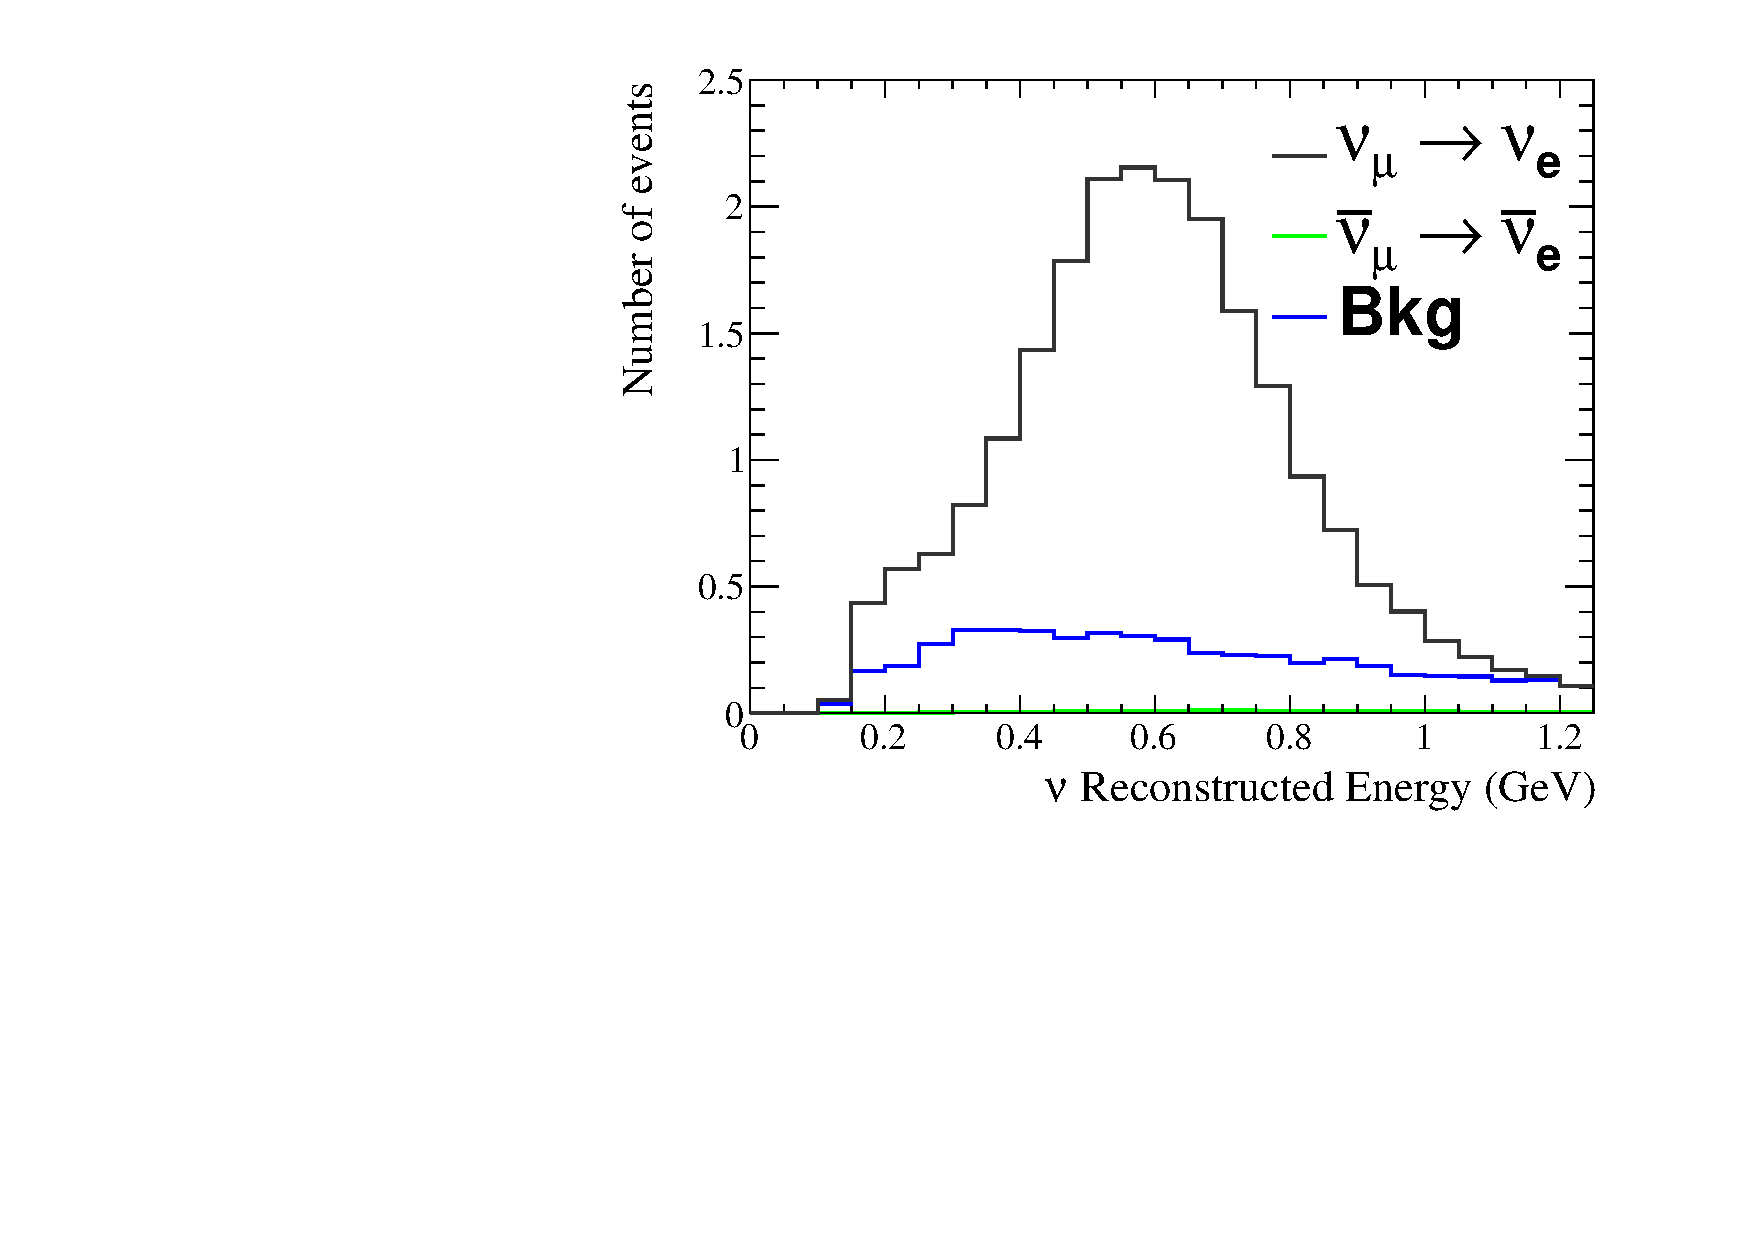
\includegraphics[width=18pc]{joint_plots/spectrum_predictions/template_ereco_1re_component.pdf}
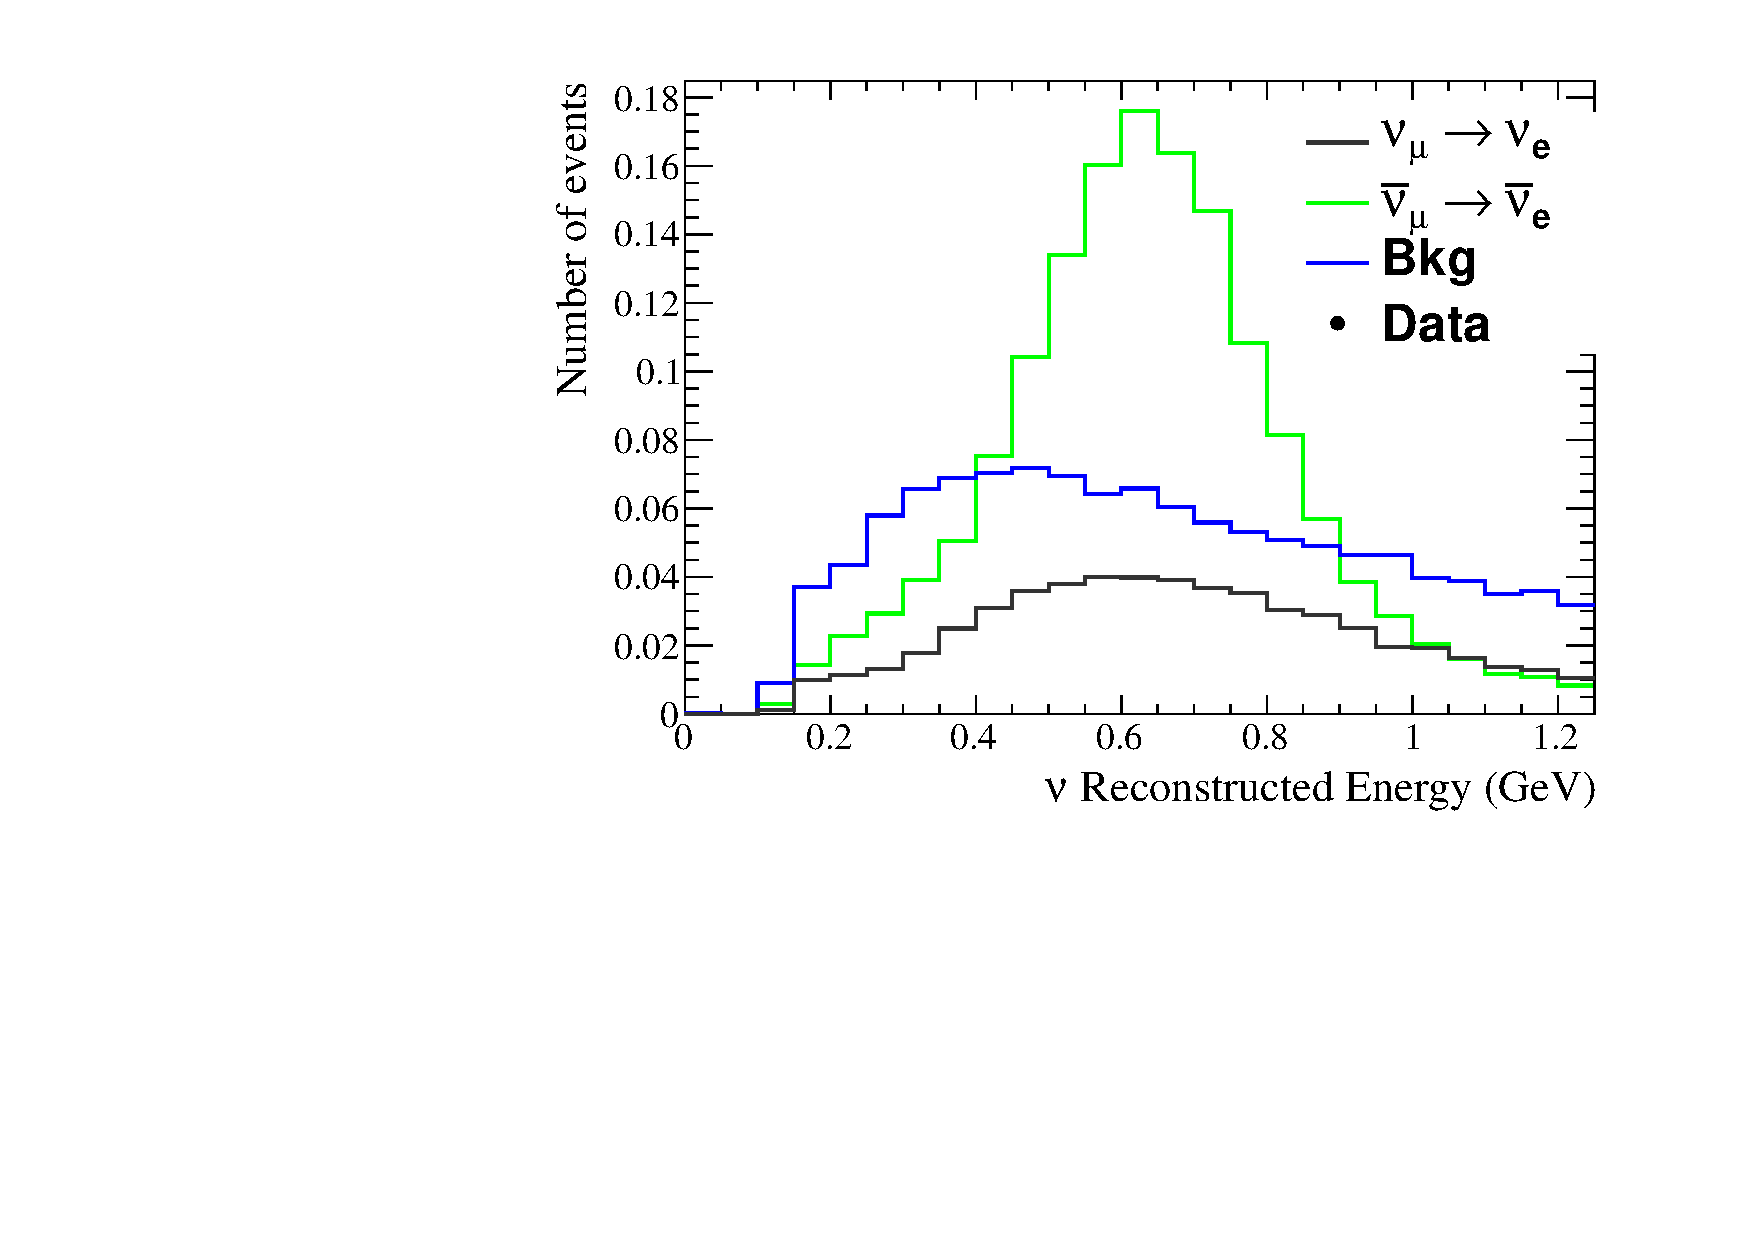
\includegraphics[width=18pc]{joint_plots/spectrum_predictions/template_ereco_rhc1re_component.pdf}
\caption {
  %  \huge{TO UPDATE} % caption is already ok
%{\large{ERECO SPECTRA WITH SEPARATED COMPONENTS}}
Predicted spectra of reconstructed neutrino energy 
for electron-like 
neutrino mode (left)
and
antineutrino mode (right)
events.
The distributions correspond to the collected statistics in the full Run 1-6 data set.
%for an exposure 
%of $6.914 \times 10^{20}$ POT in neutrino mode
%and
%of $4.011 \times 10^{20}$ POT in antineutrino mode.
The distributions are broken down by the following components:
$\bar{\nu}_{\mu} \to \bar{\nu}_e$ (green), 
$\nu_{\mu} \to \nu_e$ (black/white), 
background, 
which includes 
NC,
$\nu_e + \bar{\nu}_e$ intrinsic beam (yellow),
$\nu_{\mu}$ intrinsic beam (light blue)
and
$\bar{\nu}_{\mu}$ intrinsic beam (blue).
The spectra were generated with the systematic parameters measured with the ND280 data 
shown in \cref{tab:banff_uncertainties_flux_fhc},~\ref{tab:banff_uncertainties_flux_rhc},~\ref{tab:banff_uncertainties_xsec},
the nominal Super-K systematic parameters shown in \cref{tab:banff_uncertainties_skdetfsi}
and the oscillation parameters corresponding to the Asimov data set A shown in \cref{tab:osc_params_joint_asimov}.
It is not a stacked plot.
%The predicted spectrum of antineutrino mode 
%is scaled by a factor 7.
}
\label{fig:joint_ereco_components}
\end{figure*}


Another kinematical variable is thus needed in order to better separate different flavour / reaction compoonents.
In \cref{fig:joint_ereco_vs_theta_1re} and~\ref{fig:joint_ereco_vs_theta_rhc1re}
the 2-dimensional $E_{reco}$ vs $\theta$ spectra are shown for each flavour component and NC
for both neutrino and antineutrino mode $e$-like samples.
In particular the shapes of $\nu_{\mu} \rightarrow \nu_e$ and $\bar{\nu}_{\mu} \rightarrow \bar{\nu}_e$ 
distributions are quite different, thus this templates have a better capability to 
discriminate signal from background.
In general this template parametrization produces quite different shapes for all the main flavour and NC components.

\begin{figure*}[htb]
%\hspace{0.06\linewidth}
\center
\begin{subfigure}[b]{0.49\textwidth}
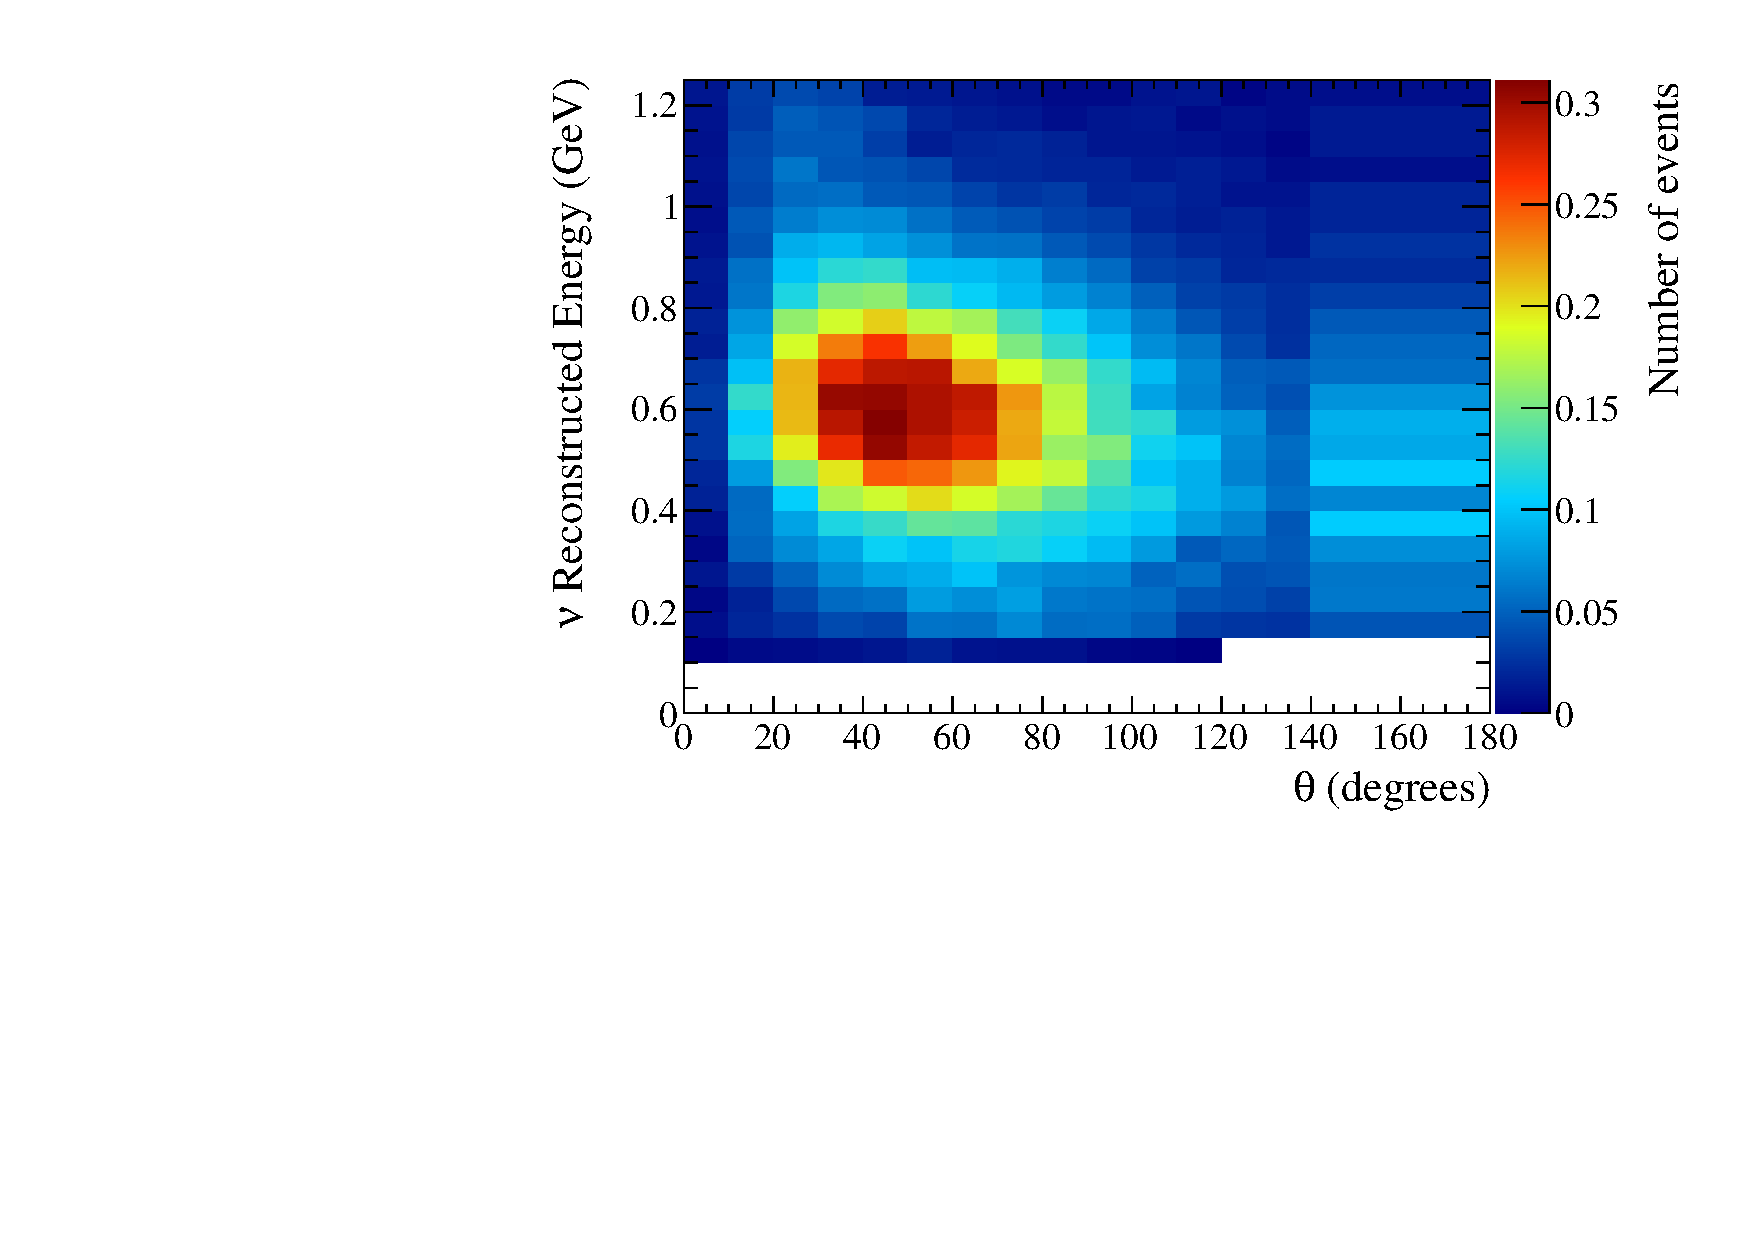
\includegraphics[width=0.9\textwidth]{joint_plots/spectrum_predictions/template_ereco_vs_theta_tot_1re.pdf}
\caption{Total}
\end{subfigure}\\
\begin{subfigure}[b]{0.49\textwidth}
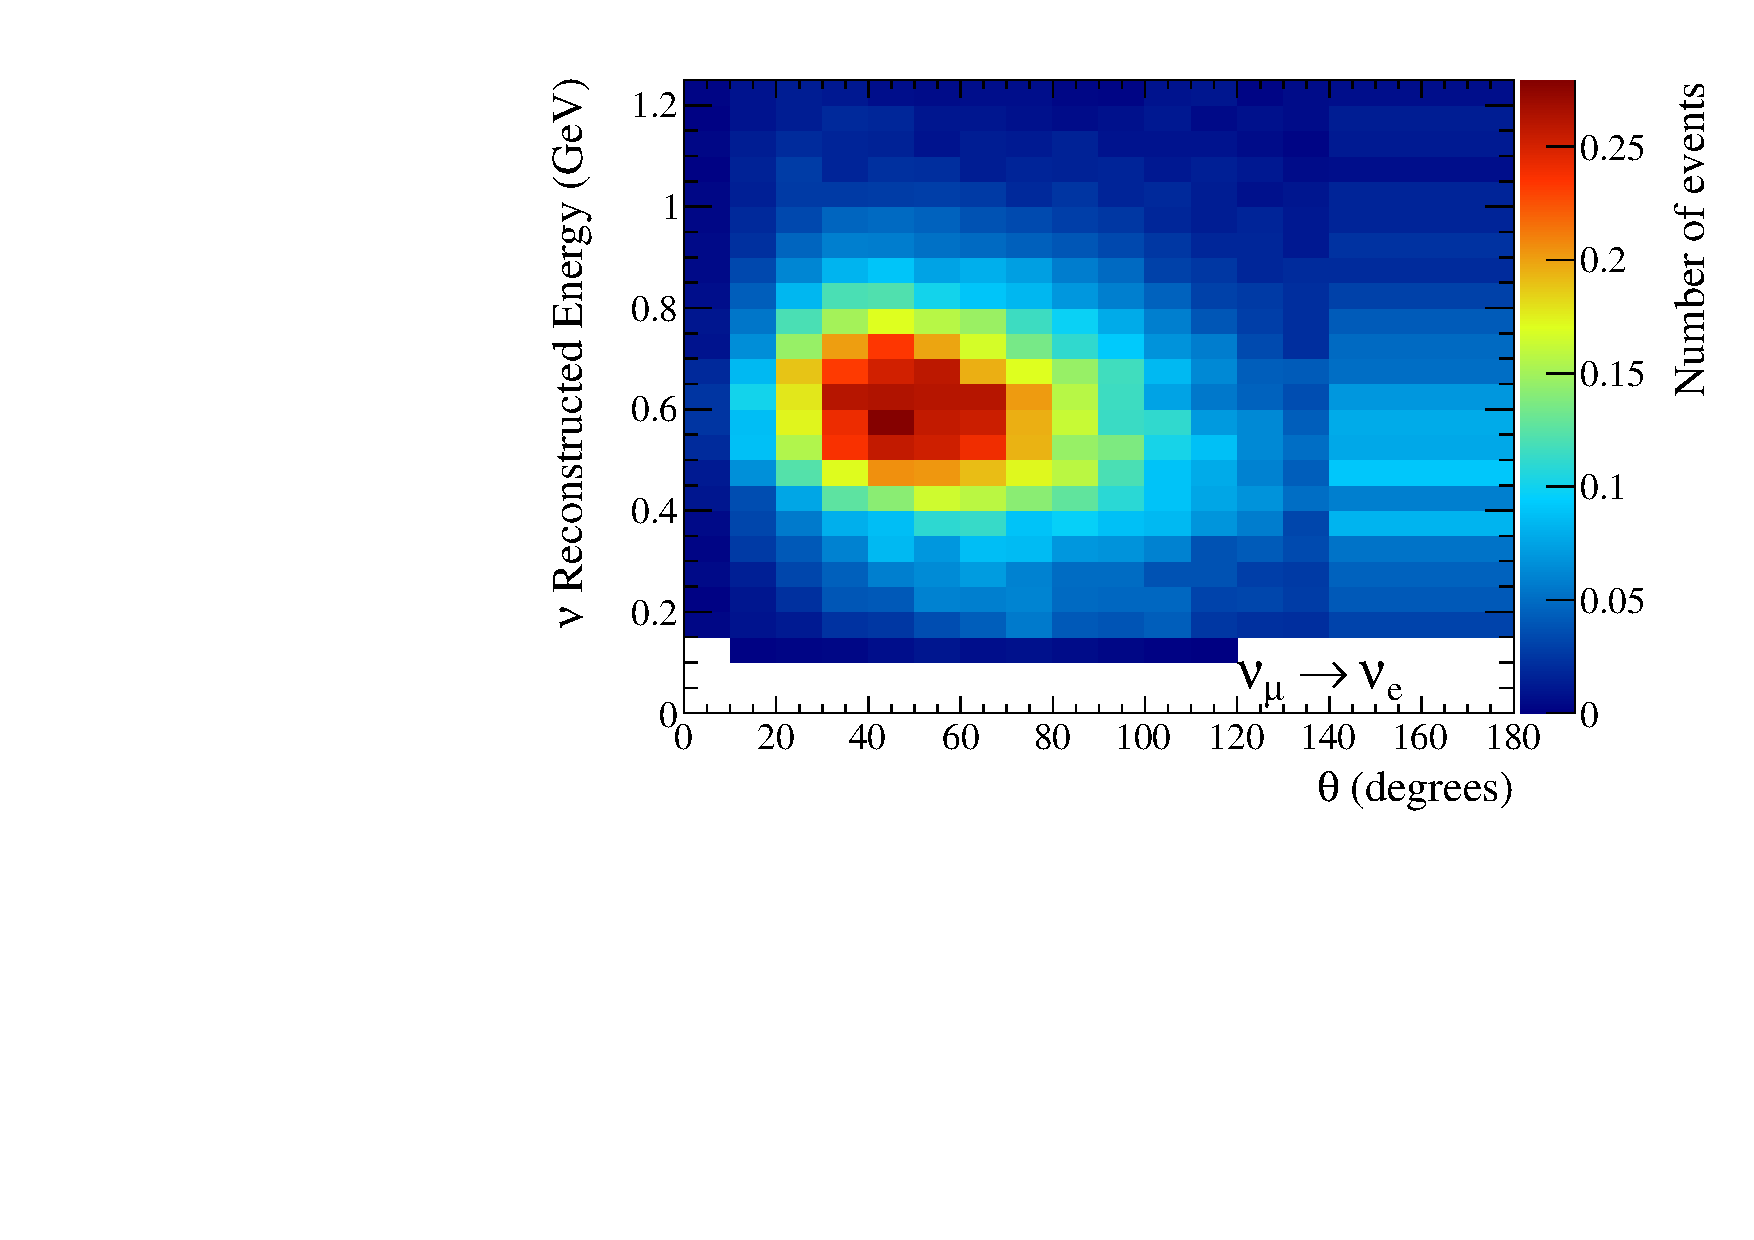
\includegraphics[width=0.9\textwidth]{joint_plots/spectrum_predictions/template_ereco_vs_theta_numutonue_1re.pdf}
\caption{$\nu_{\mu} \rightarrow \nu_e$.}
\end{subfigure}
\begin{subfigure}[b]{0.49\textwidth}
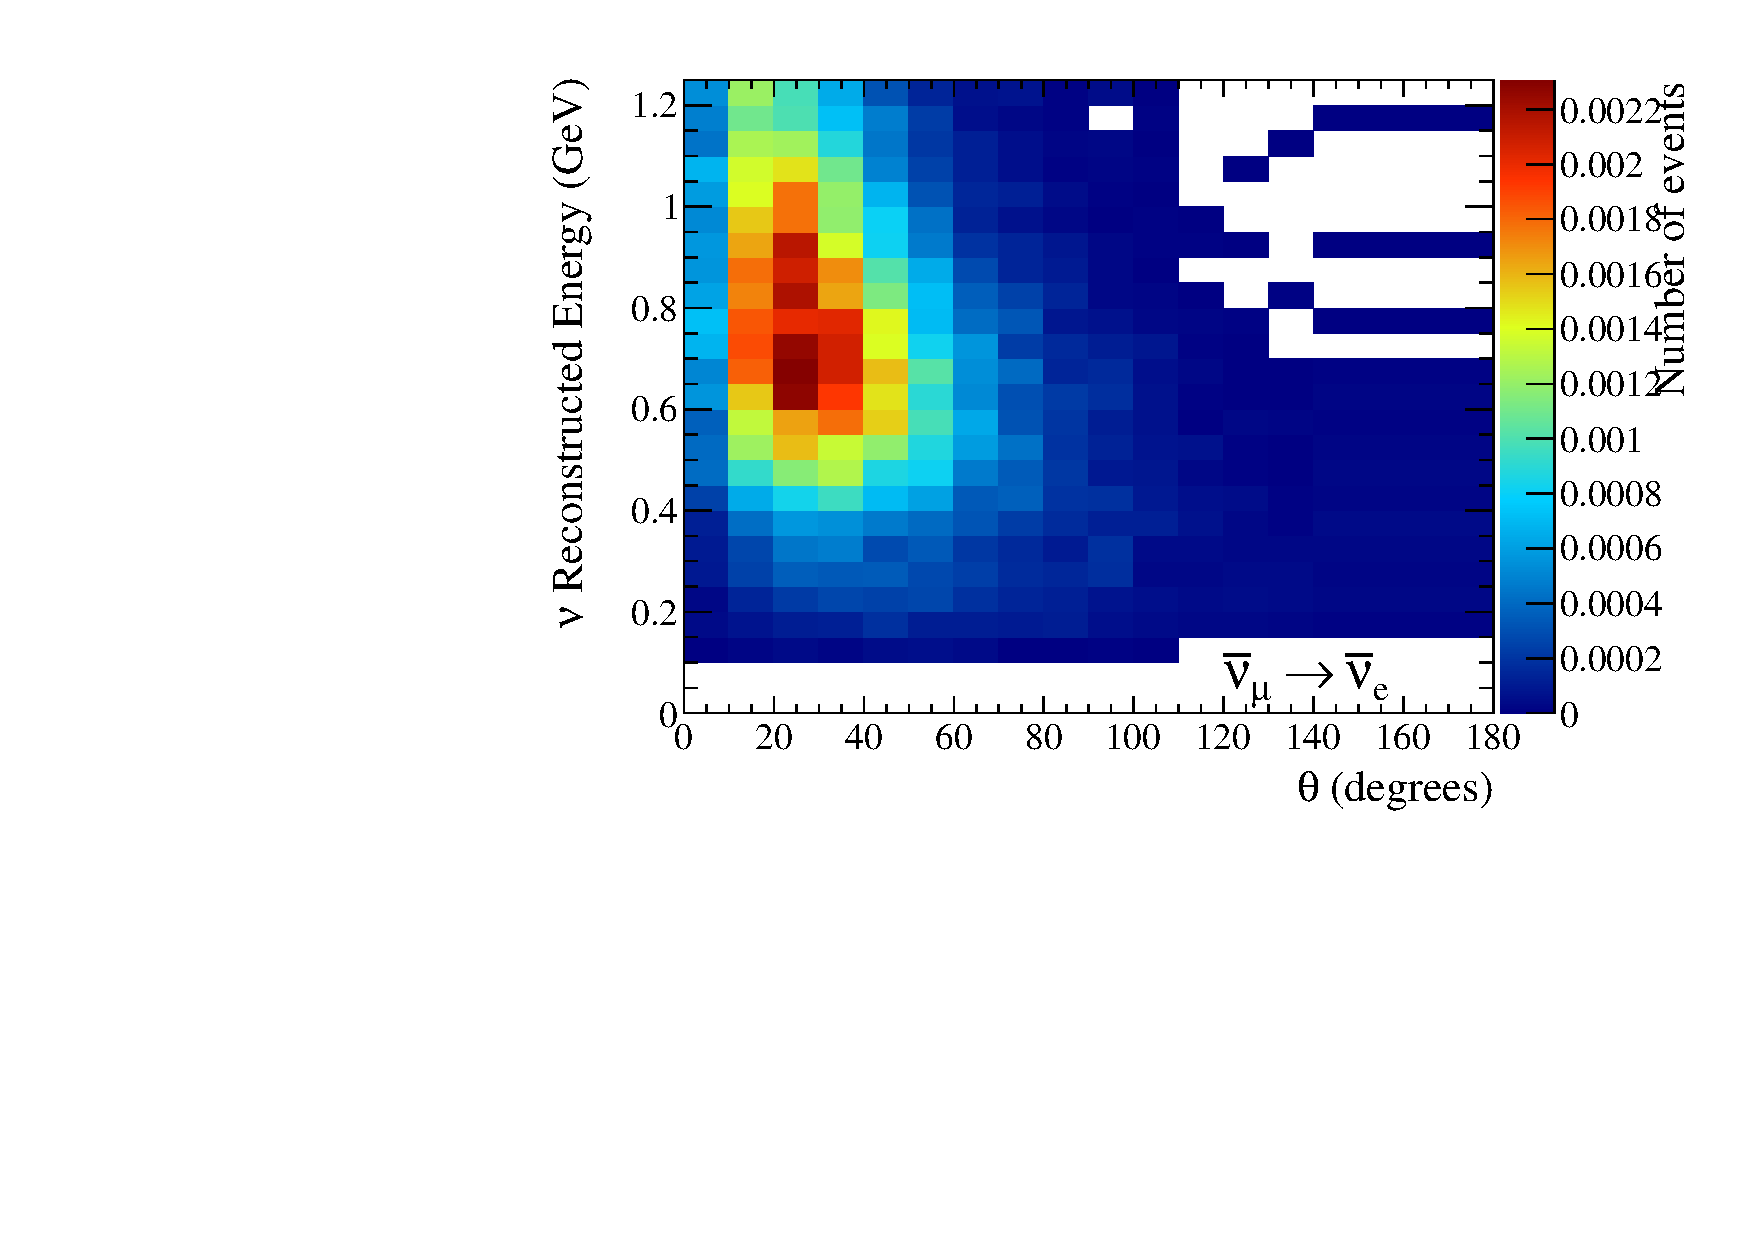
\includegraphics[width=0.9\textwidth]{joint_plots/spectrum_predictions/template_ereco_vs_theta_numubartonuebar_1re.pdf}
\caption{$\bar{\nu}_{\mu} \rightarrow \bar{\nu}_e$.}
\end{subfigure}
\begin{subfigure}[b]{0.49\textwidth}
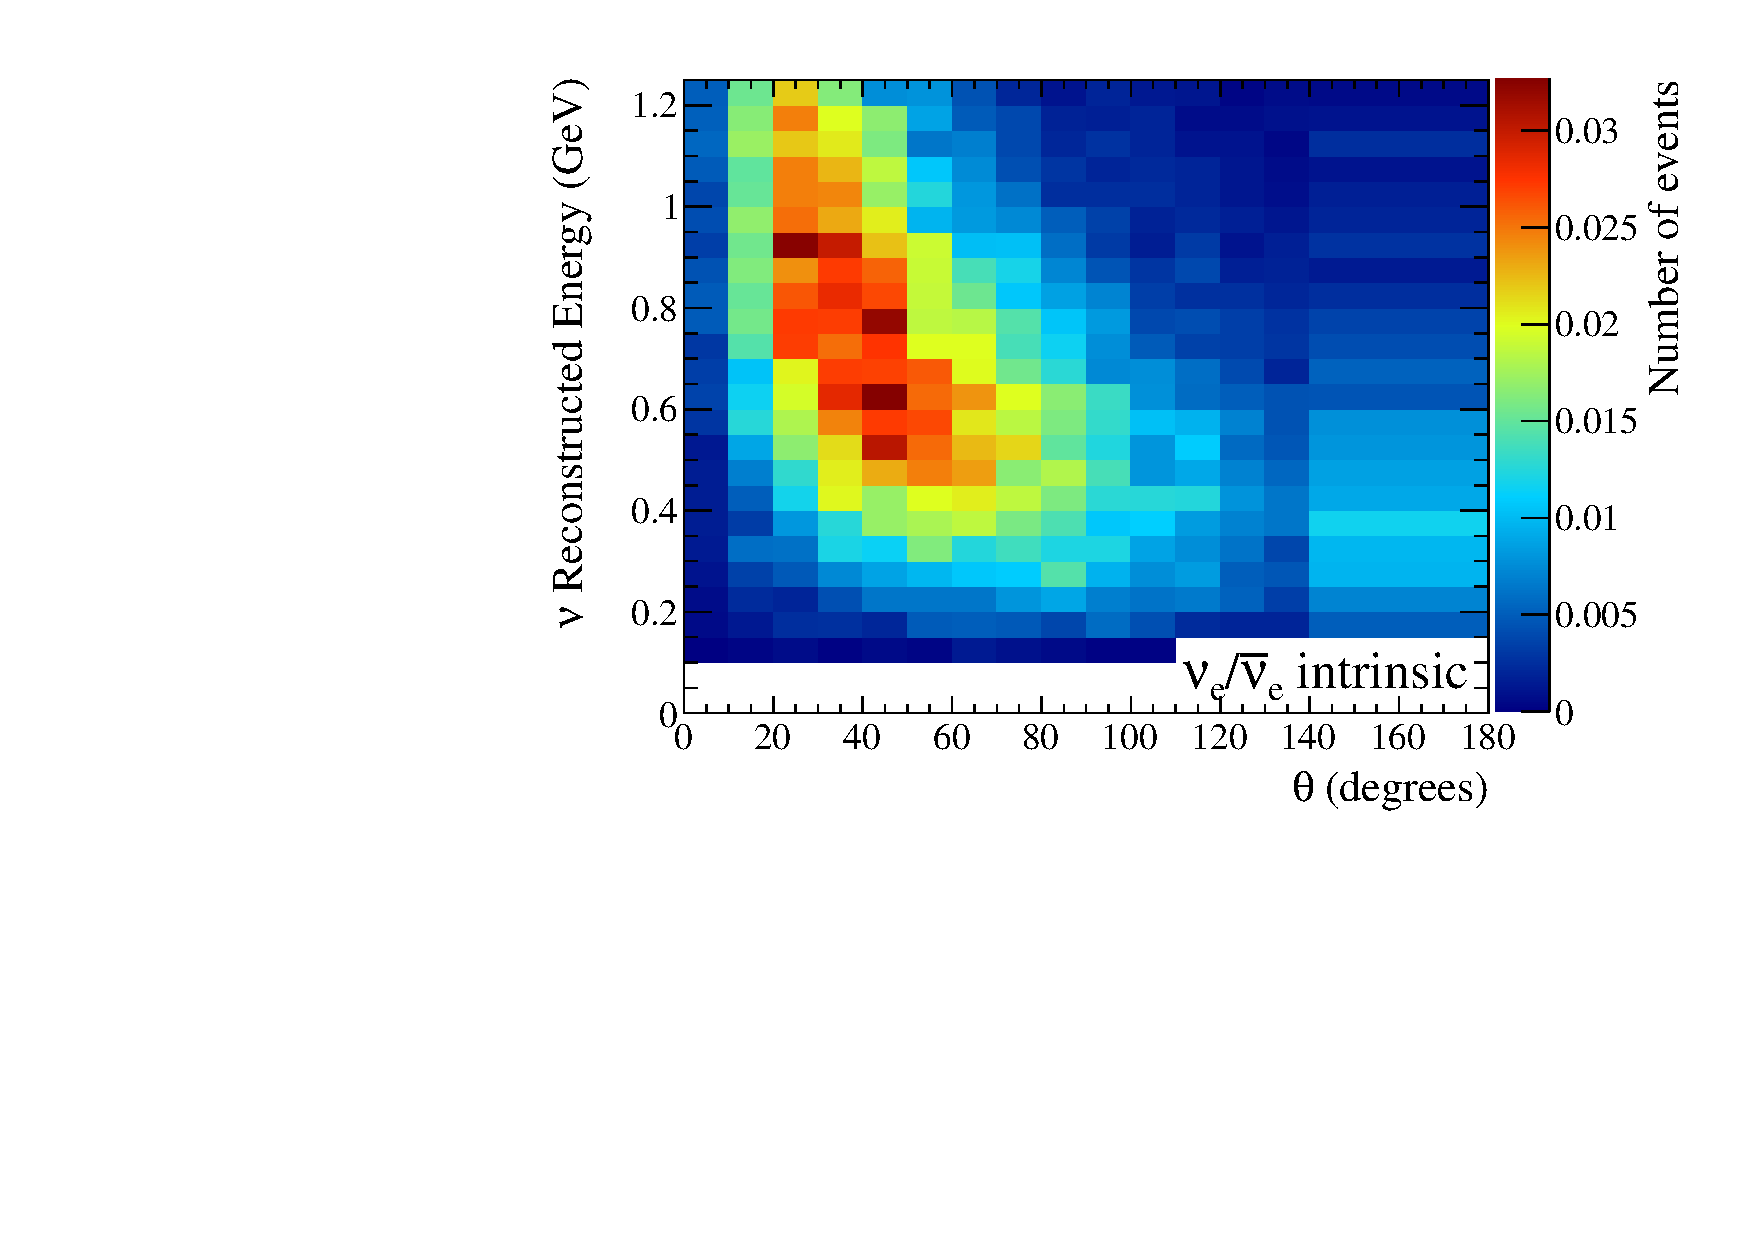
\includegraphics[width=0.9\textwidth]{joint_plots/spectrum_predictions/template_ereco_vs_theta_nuebeam_1re.pdf}
\caption{$\nu_{e}$ + $\bar{\nu}_e$ intrinsic beam.}
\end{subfigure}
\begin{subfigure}[b]{0.49\textwidth}
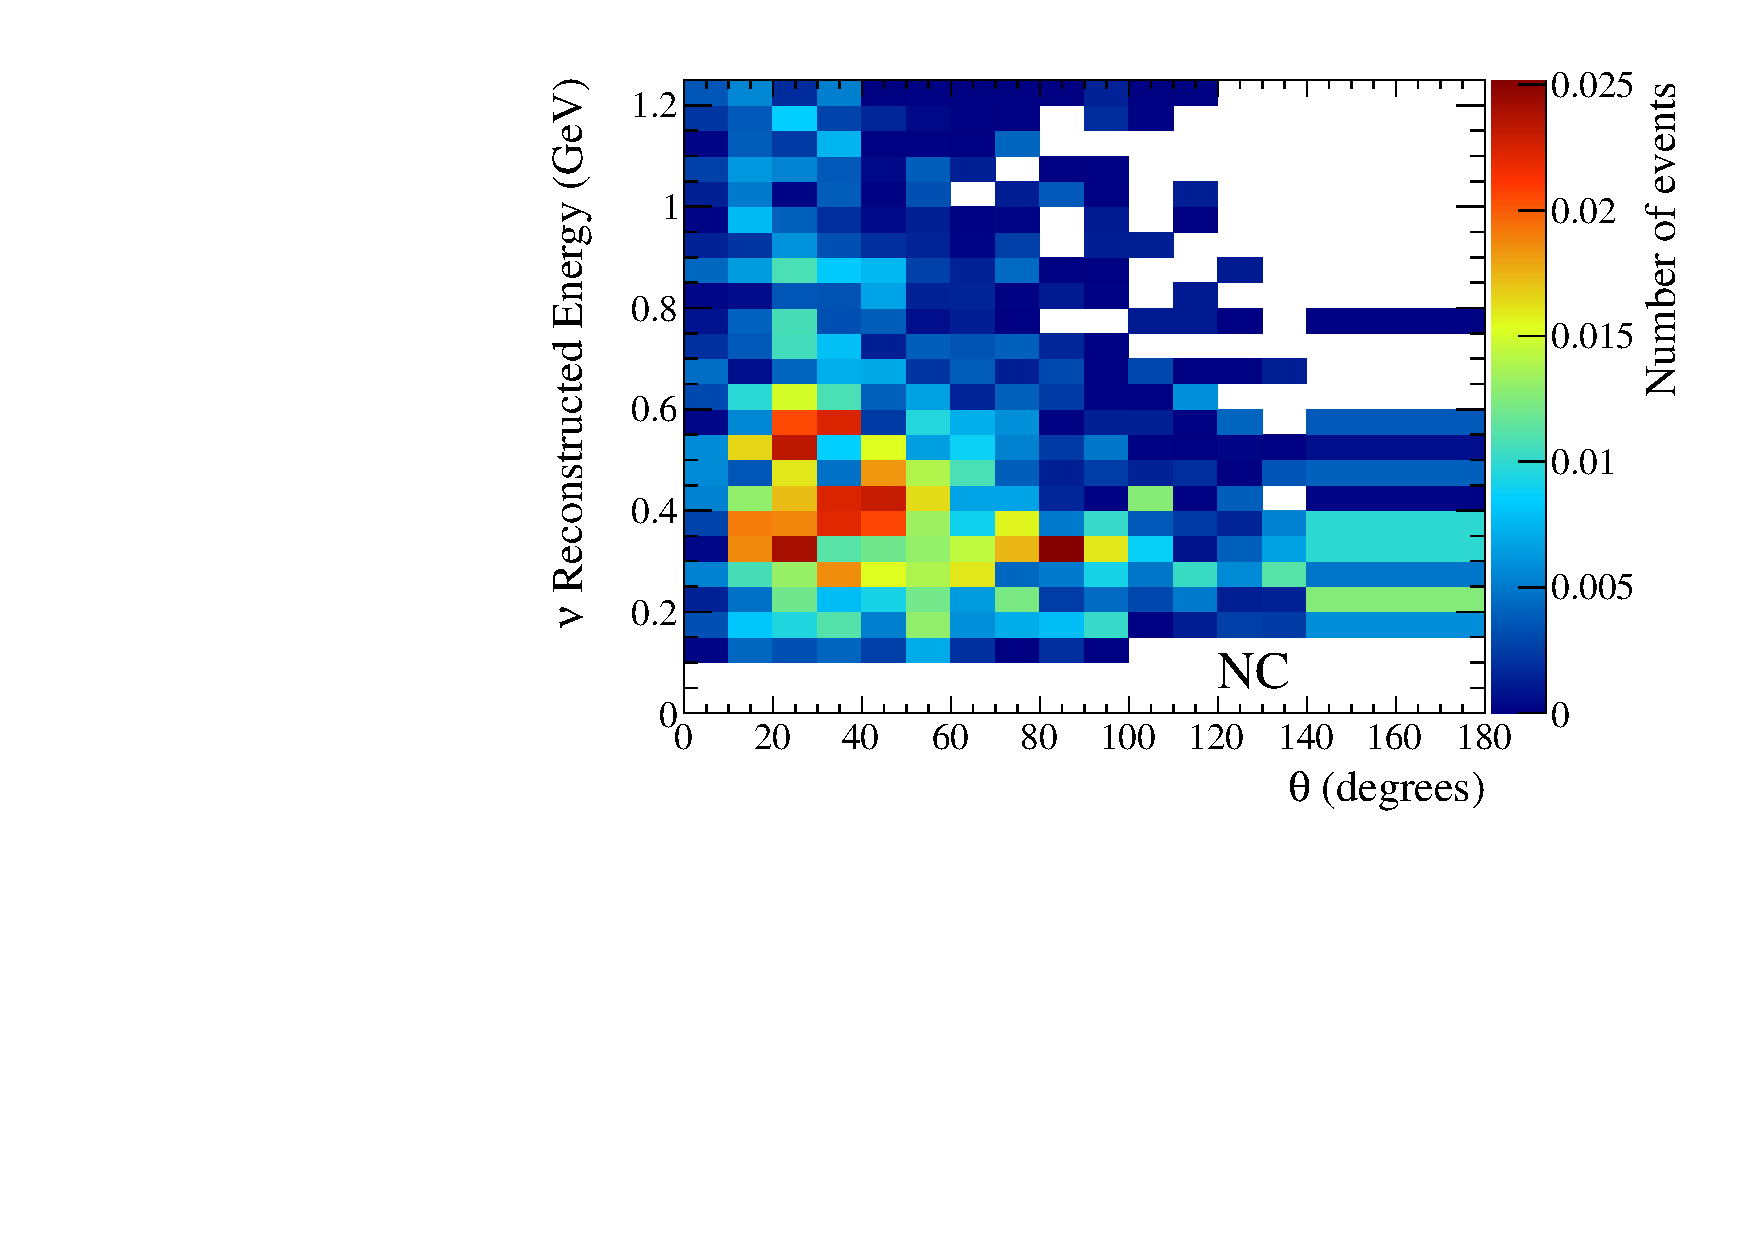
\includegraphics[width=0.9\textwidth]{joint_plots/spectrum_predictions/template_ereco_vs_theta_nc_1re.pdf}
\caption{Neutral current.}
\end{subfigure}
\begin{subfigure}[b]{0.49\textwidth}
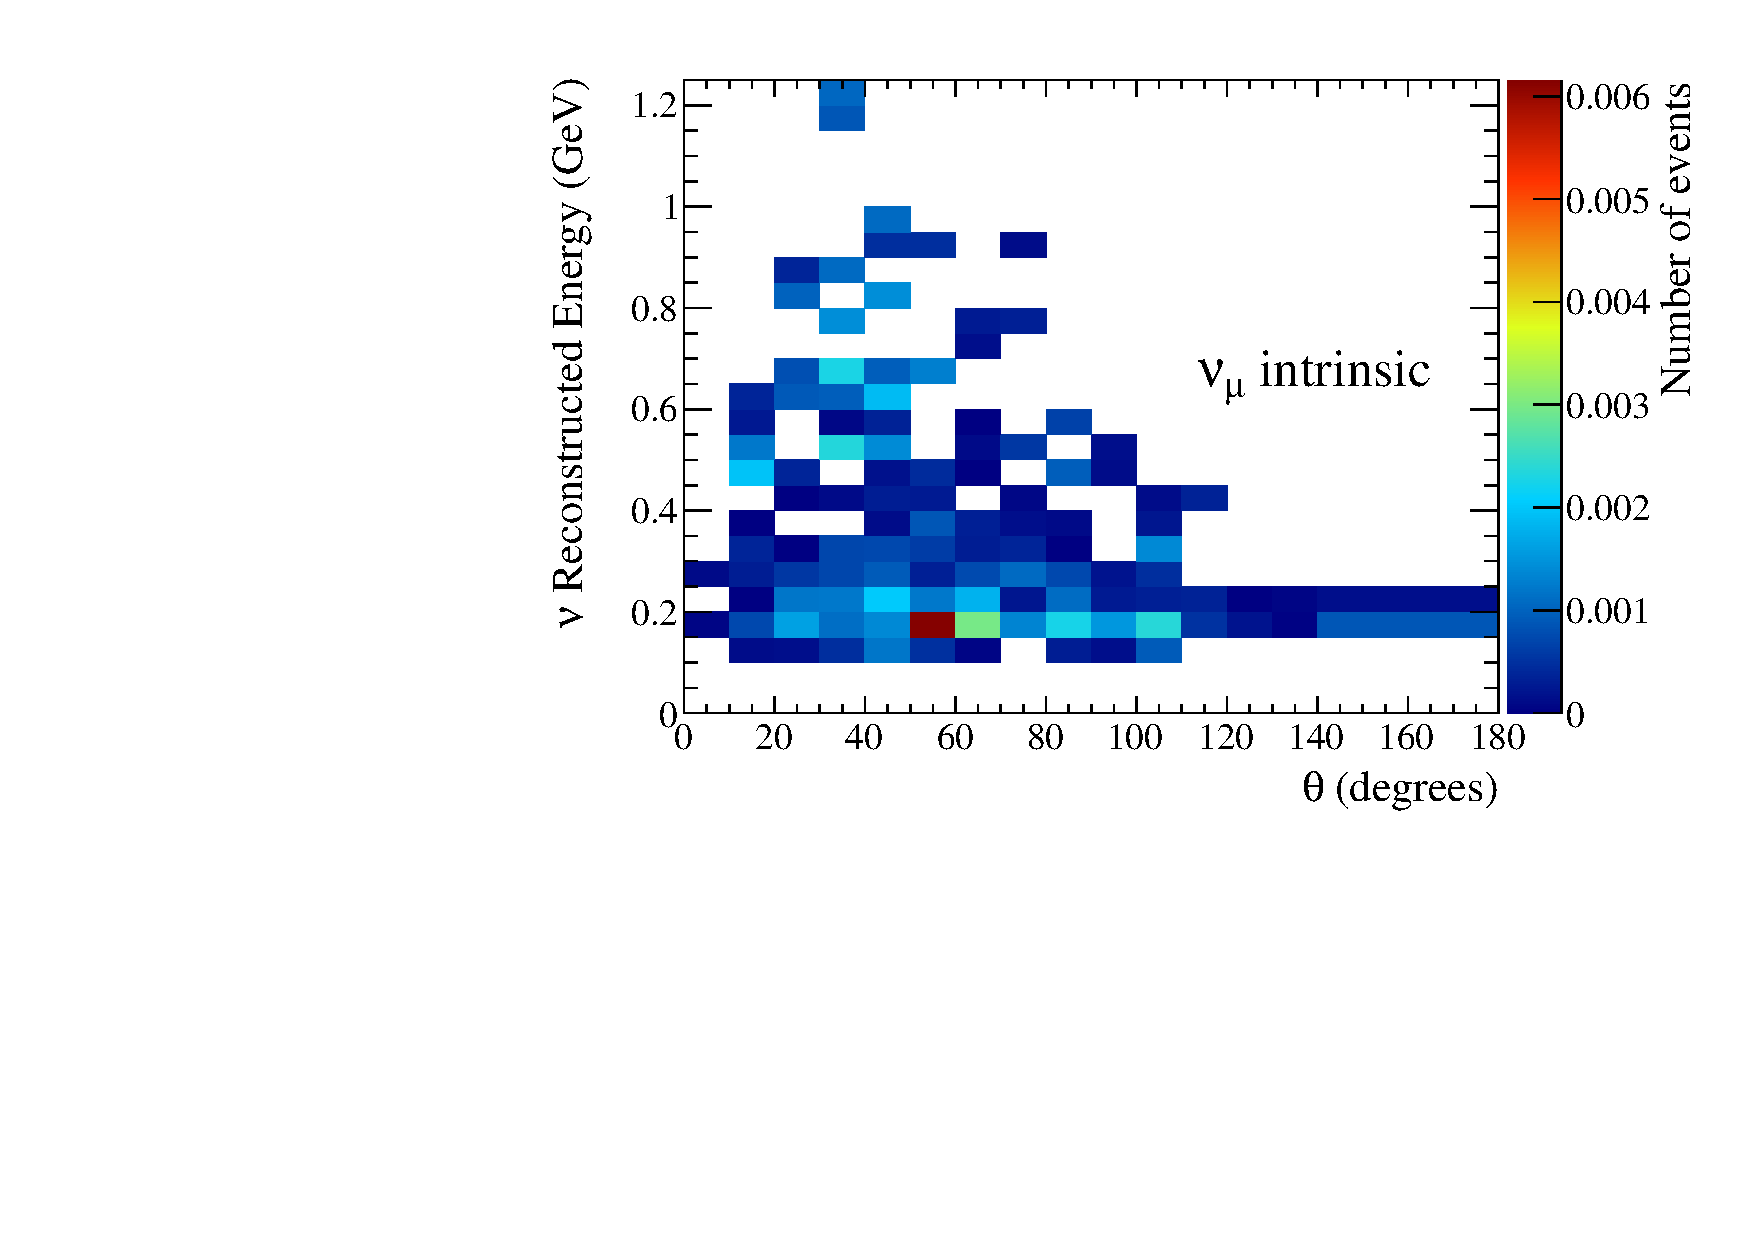
\includegraphics[width=0.9\textwidth]{joint_plots/spectrum_predictions/template_ereco_vs_theta_numubeam_1re.pdf}
\caption{$\nu_{\mu}$ intrinsic beam.}
\end{subfigure}
\begin{subfigure}[b]{0.49\textwidth}
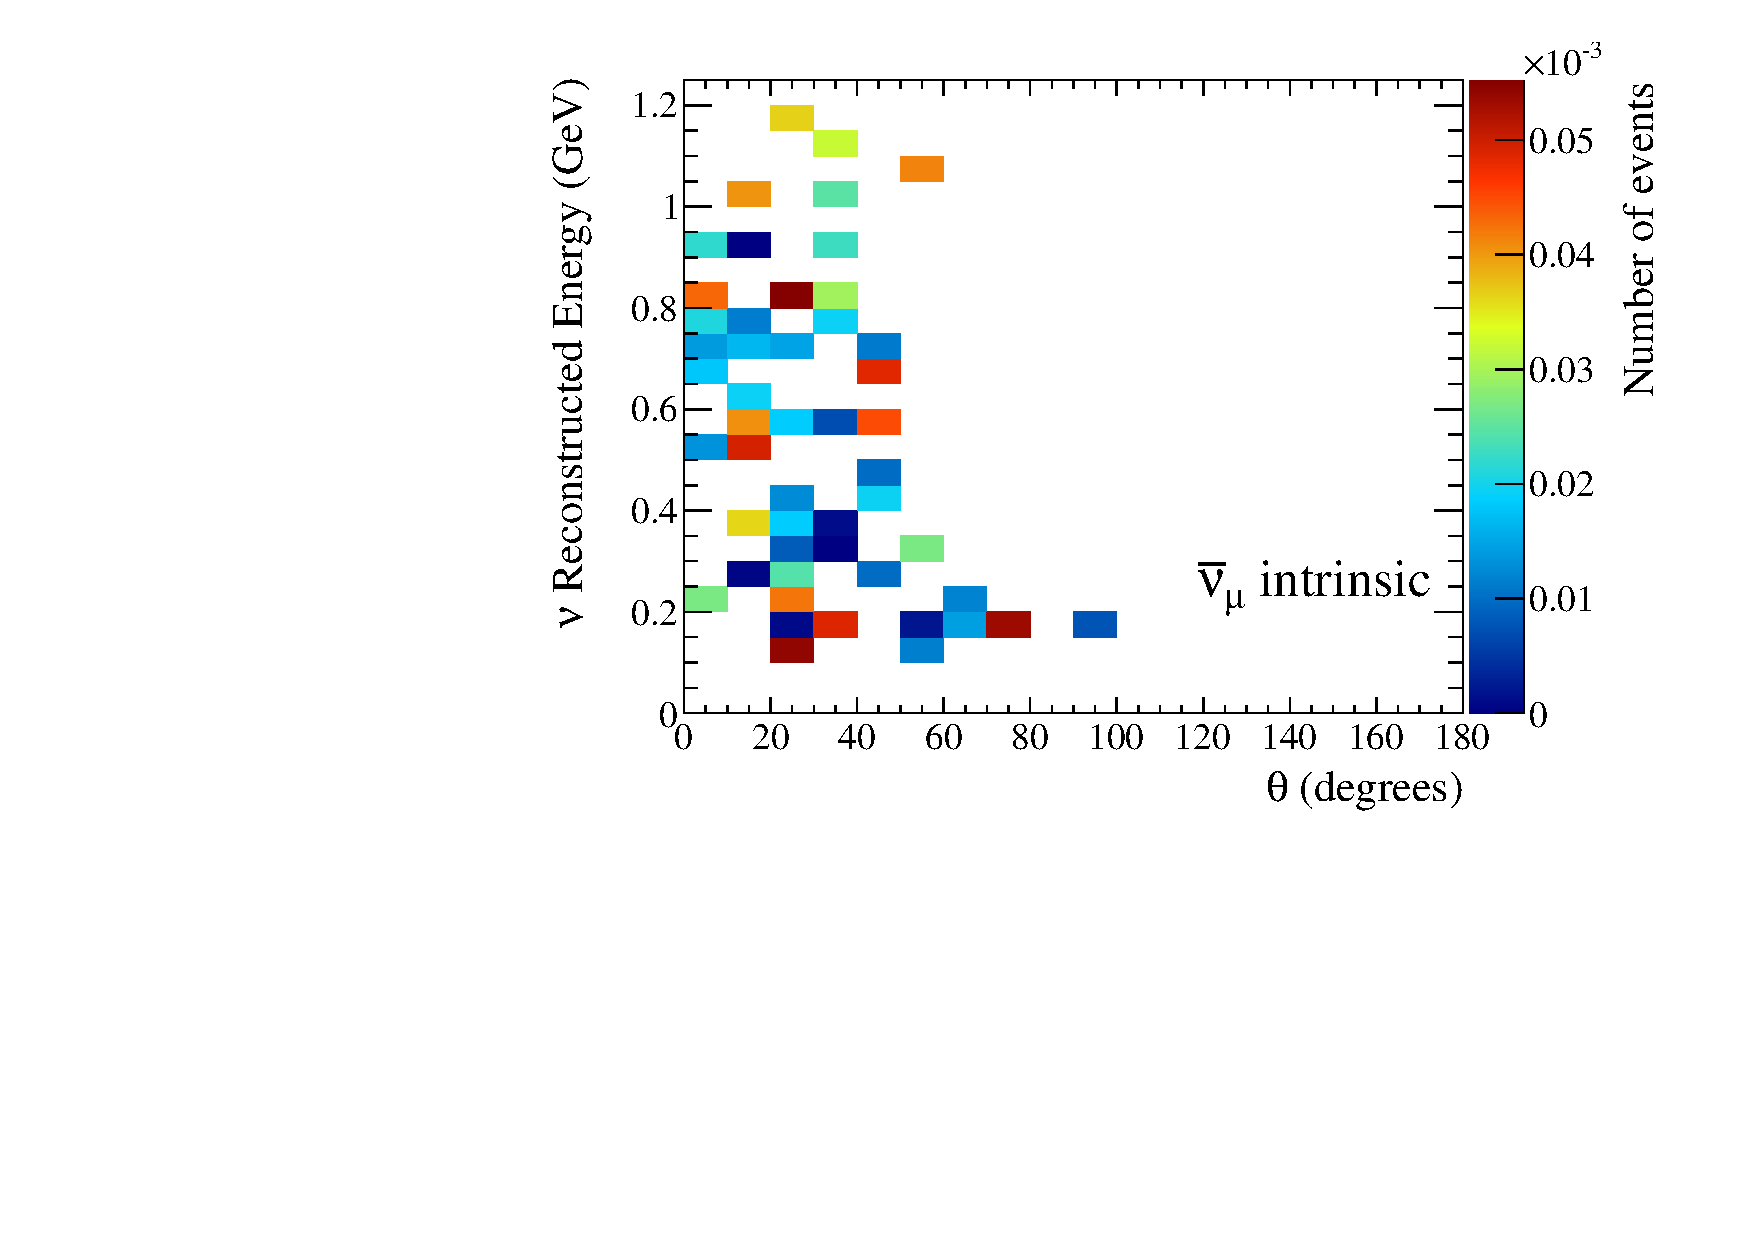
\includegraphics[width=0.9\textwidth]{joint_plots/spectrum_predictions/template_ereco_vs_theta_numubarbeam_1re.pdf}
\caption{$\bar{\nu}_{\mu}$ intrinsic beam.}
\end{subfigure}
\caption {
Predicted spectra of electron-like events
as a function of the reconstructed neutrino energy and
the angle between the outgoing lepton and the neutrino direction.
The distributions correspond to the collected statistics in the full Run 1-6 data set.
%for an exposure 
%of $6.914 \times 10^{20}$ POT in neutrino mode.
%and
%of $4.011 \times 10^{20}$ POT in antineutrino mode.
From top left to bottom right the following components are shown:
total,
$\nu_{\mu} \rightarrow \nu_e$,
$\bar{\nu}_{\mu} \rightarrow \bar{\nu}_e$,
$\nu_e + \bar{\nu}_e$ intrinsic beam,
NC,
$\nu_{\mu}$ intrinsic beam
and
$\bar{\nu}_{\mu}$ intrinsic beam.
The spectra were generated with the systematic parameters measured with the ND280 data 
shown in \cref{tab:banff_uncertainties_flux_fhc},~\ref{tab:banff_uncertainties_flux_rhc},~\ref{tab:banff_uncertainties_xsec},
the nominal Super-K systematic parameters shown in \cref{tab:banff_uncertainties_skdetfsi}
and the oscillation parameters corresponding to the Asimov data set A shown in \cref{tab:osc_params_joint_asimov}.
}
\label{fig:joint_ereco_vs_theta_1re}
\end{figure*}

\begin{figure*}[htb]
%\hspace{0.06\linewidth}
\center
\begin{subfigure}[b]{0.49\textwidth}
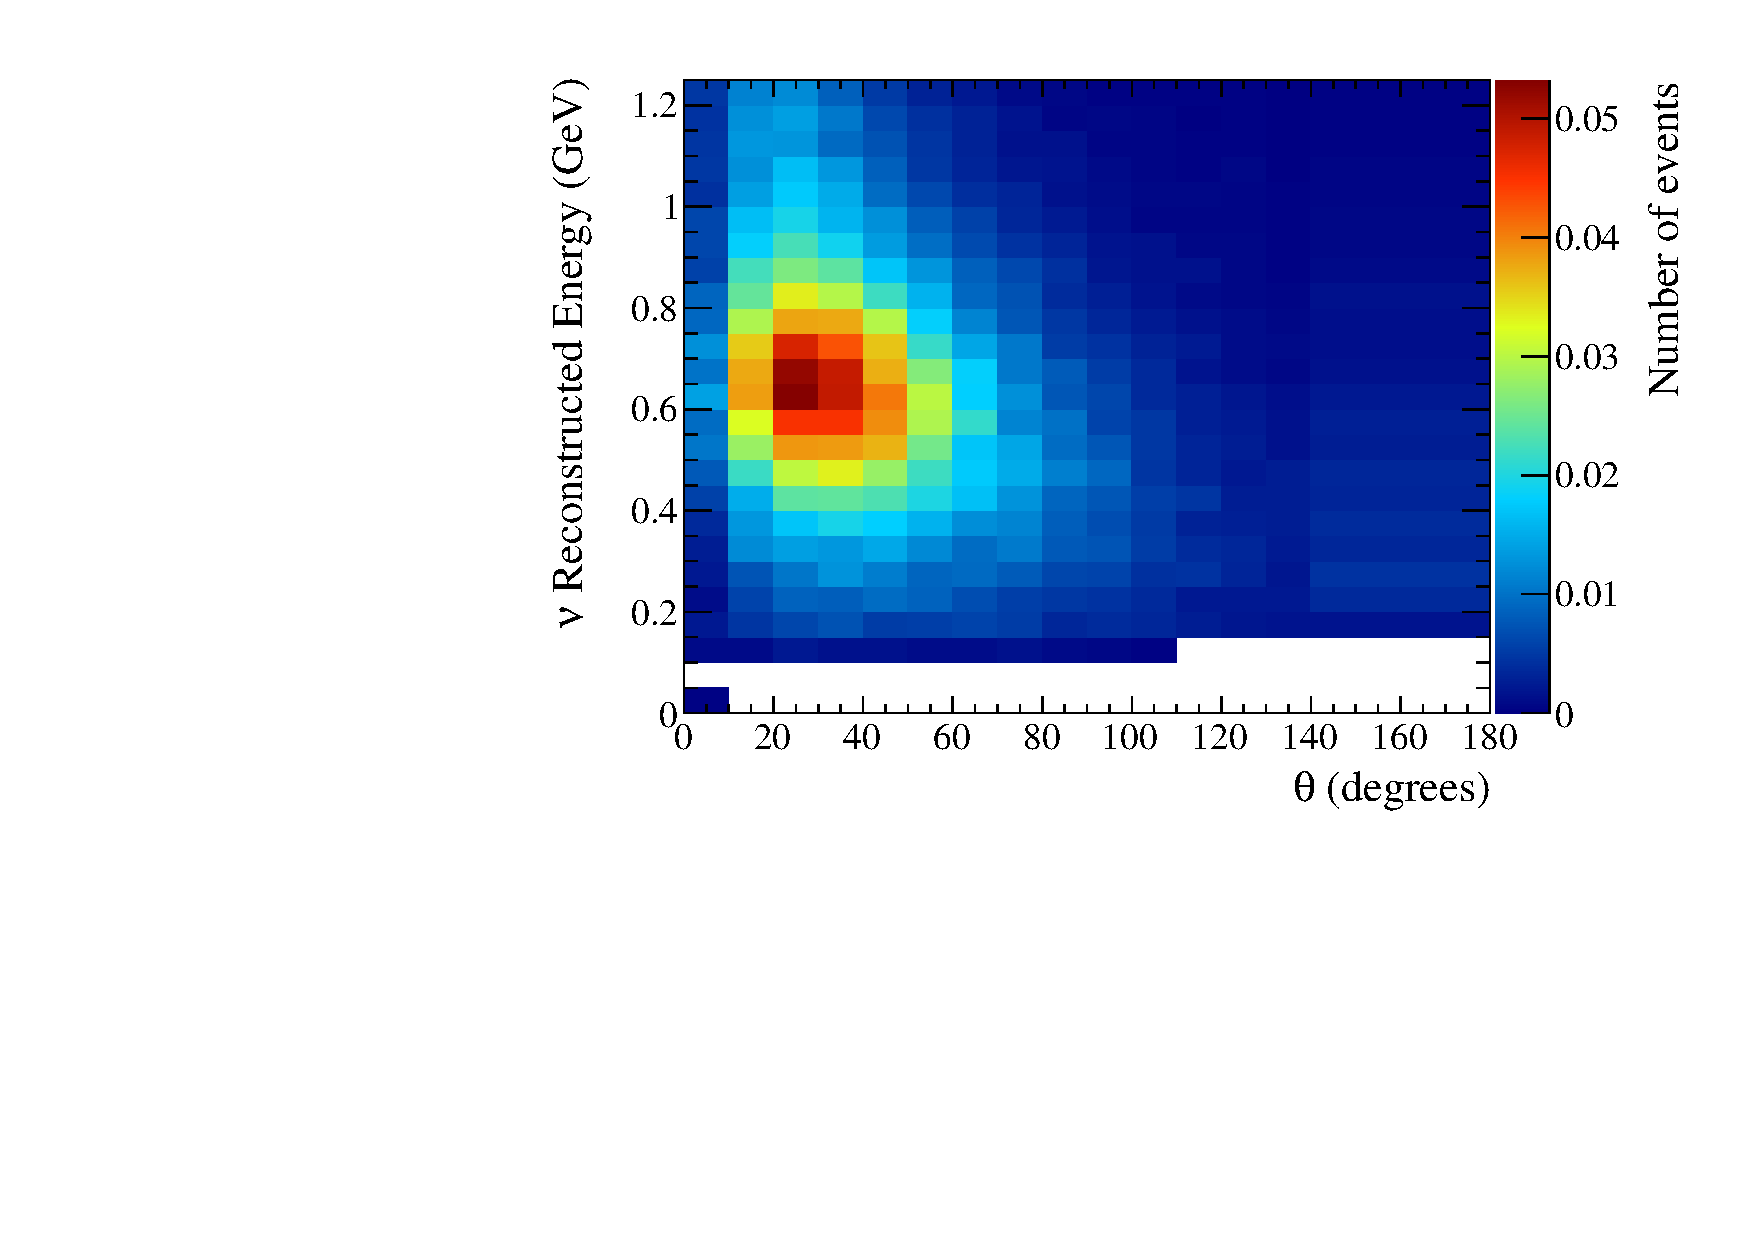
\includegraphics[width=0.9\textwidth]{joint_plots/spectrum_predictions/template_ereco_vs_theta_tot_rhc1re.pdf}\\
\caption{Total}
\end{subfigure}\\
\begin{subfigure}[b]{0.49\textwidth}
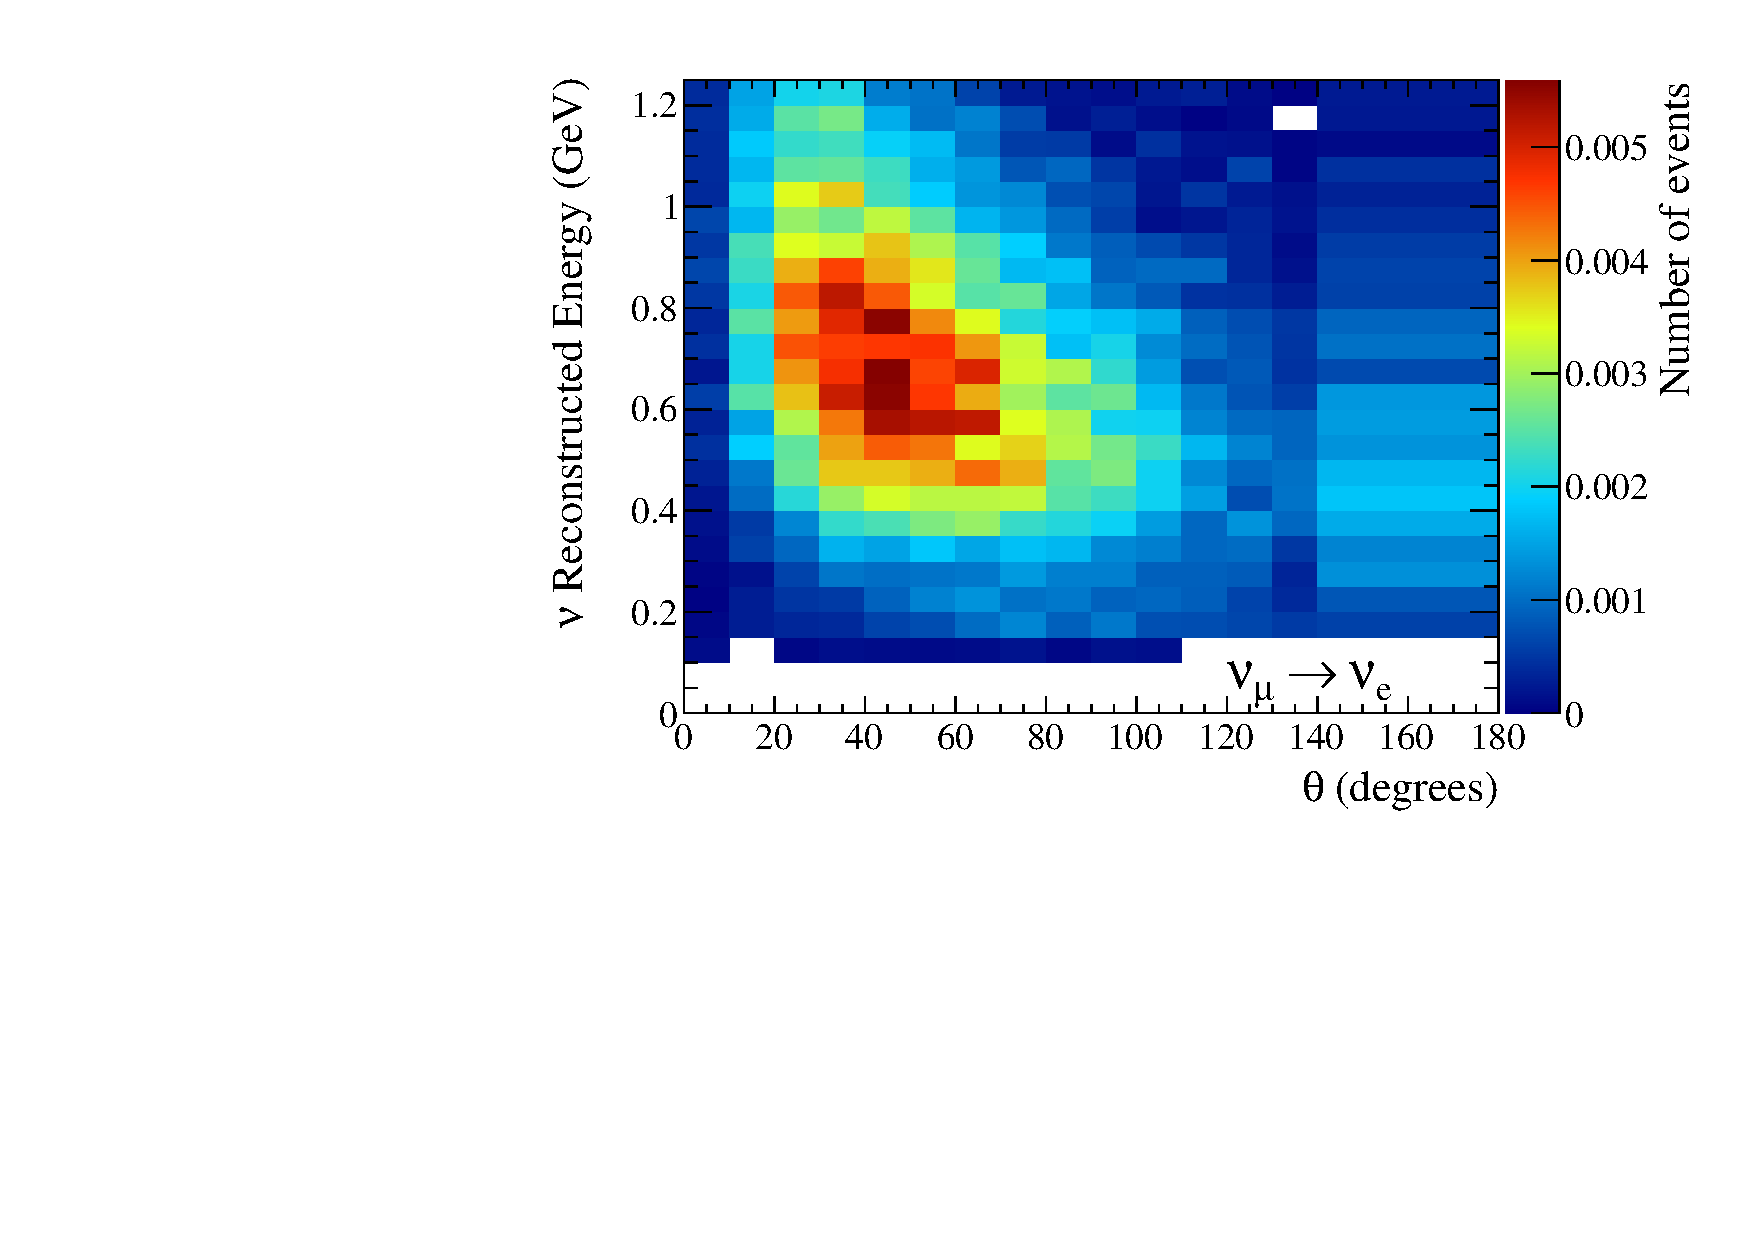
\includegraphics[width=0.9\textwidth]{joint_plots/spectrum_predictions/template_ereco_vs_theta_numutonue_rhc1re.pdf}
\caption{$\nu_{\mu} \rightarrow \nu_e$.}
\end{subfigure}
\begin{subfigure}[b]{0.49\textwidth}
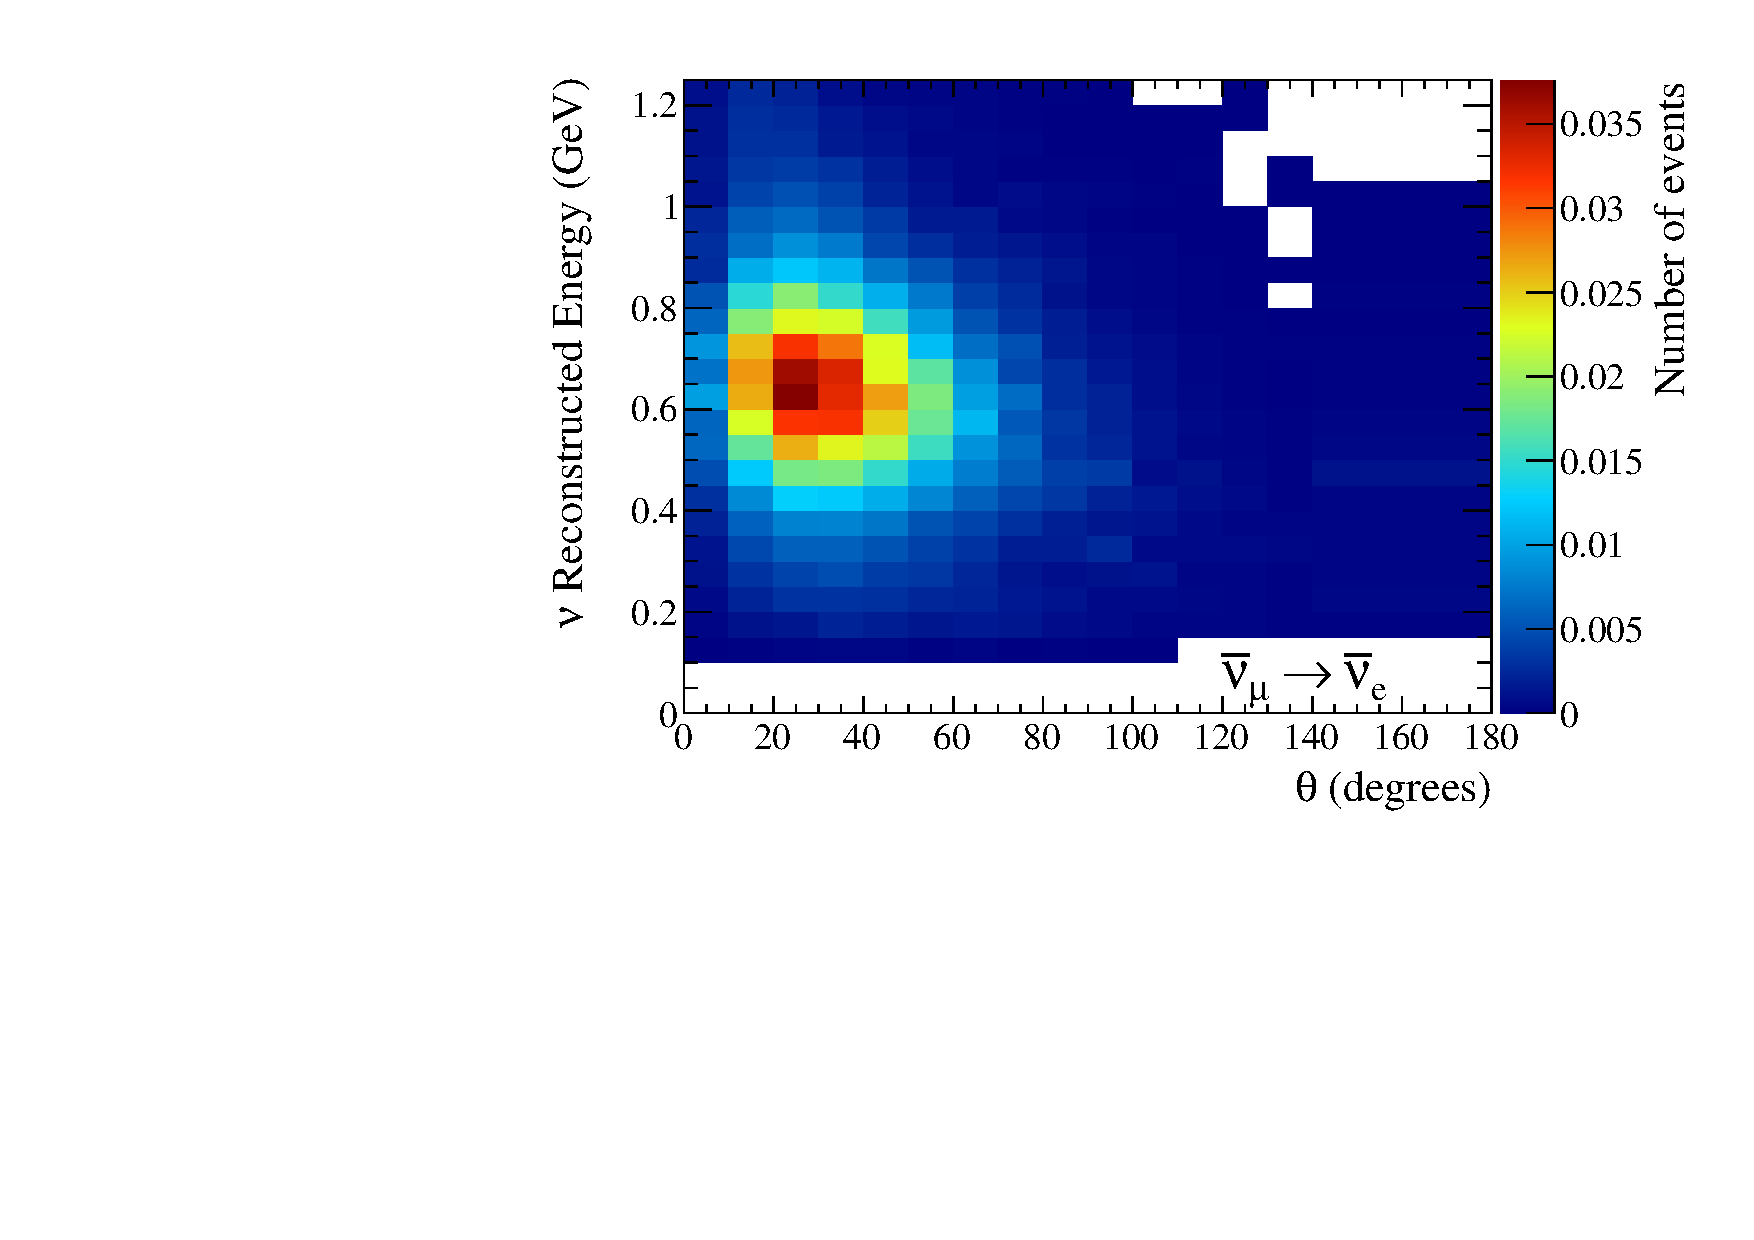
\includegraphics[width=0.9\textwidth]{joint_plots/spectrum_predictions/template_ereco_vs_theta_numubartonuebar_rhc1re.pdf}
\caption{$\bar{\nu}_{\mu} \rightarrow \bar{\nu}_e$.}
\end{subfigure}
\begin{subfigure}[b]{0.49\textwidth}
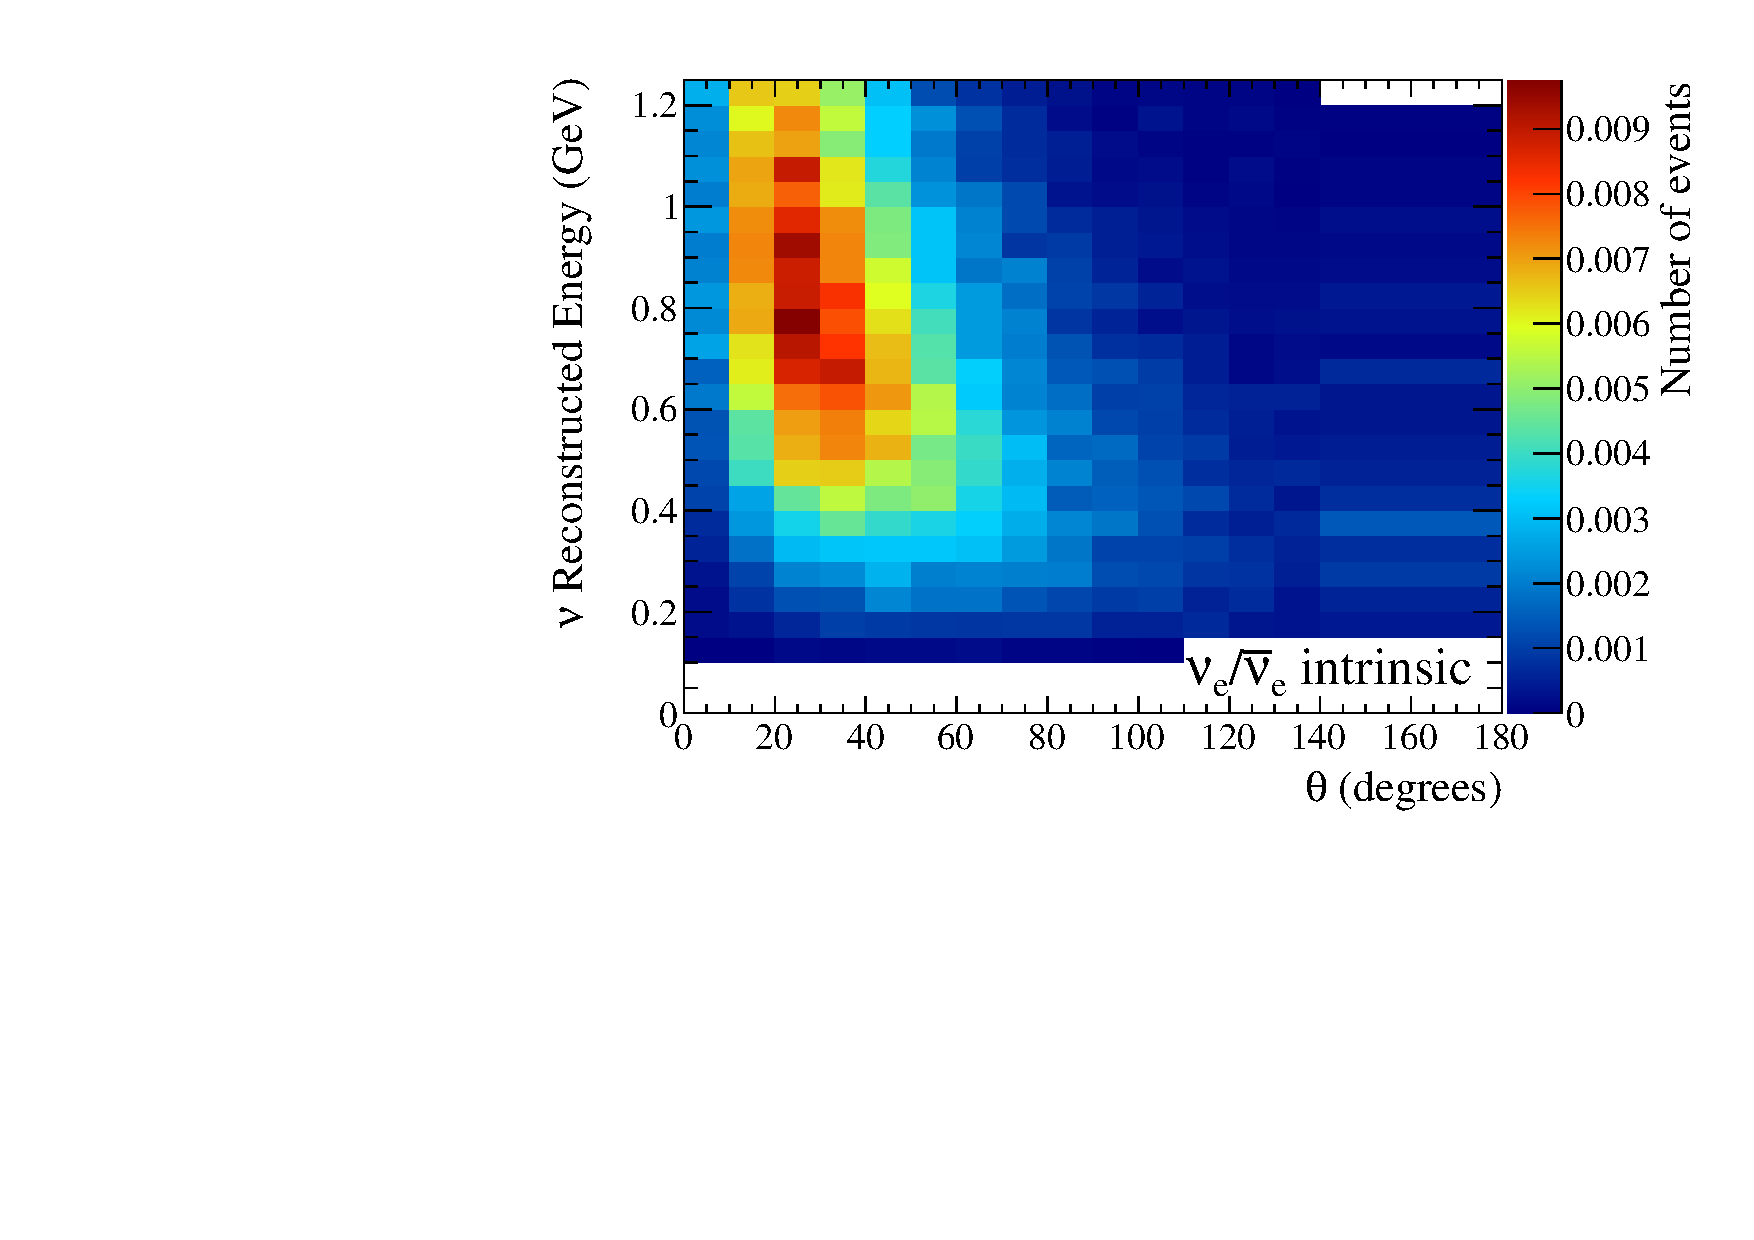
\includegraphics[width=0.9\textwidth]{joint_plots/spectrum_predictions/template_ereco_vs_theta_nuebeam_rhc1re.pdf}
\caption{$\nu_{e}$ + $\bar{\nu}_e$ intrinsic beam.}
\end{subfigure}
\begin{subfigure}[b]{0.49\textwidth}
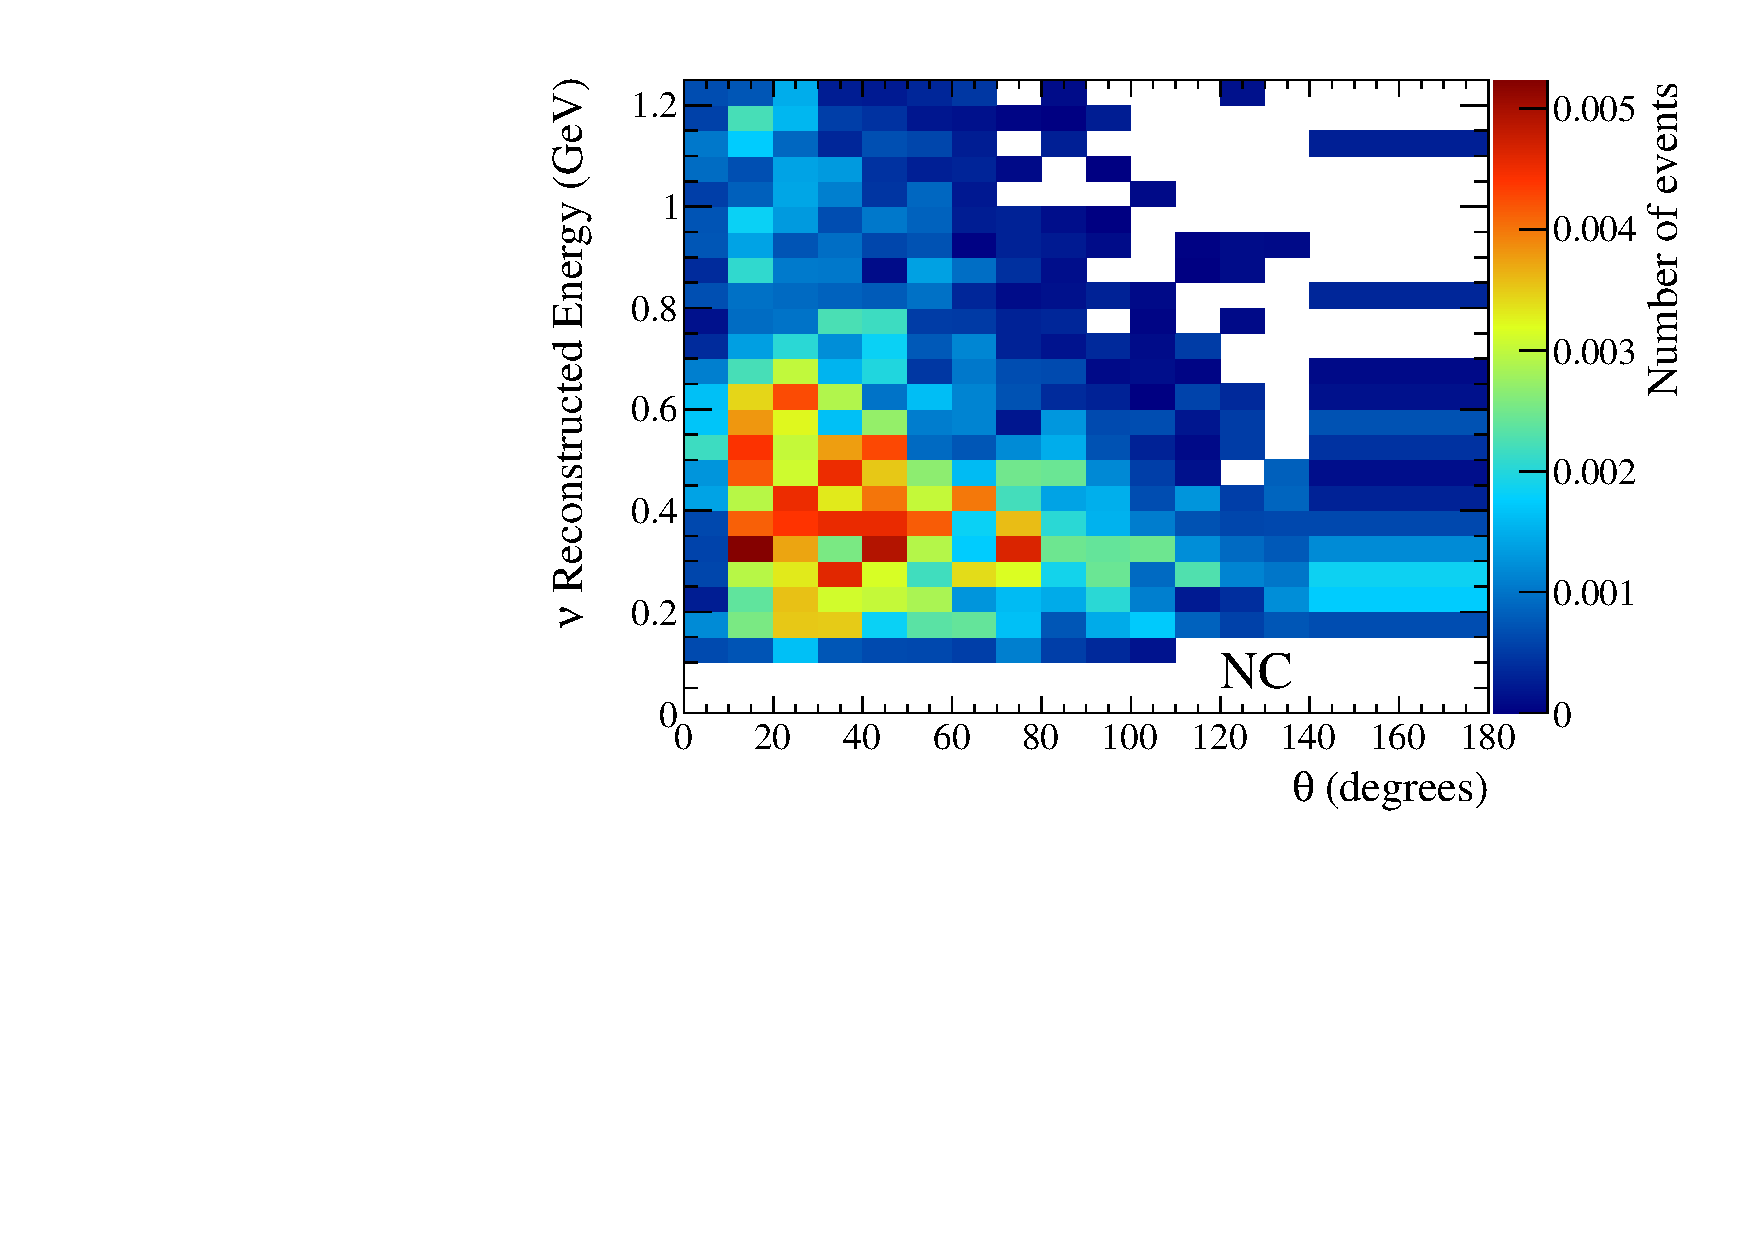
\includegraphics[width=0.9\textwidth]{joint_plots/spectrum_predictions/template_ereco_vs_theta_nc_rhc1re.pdf}
\caption{Neutral current.}
\end{subfigure}
\begin{subfigure}[b]{0.49\textwidth}
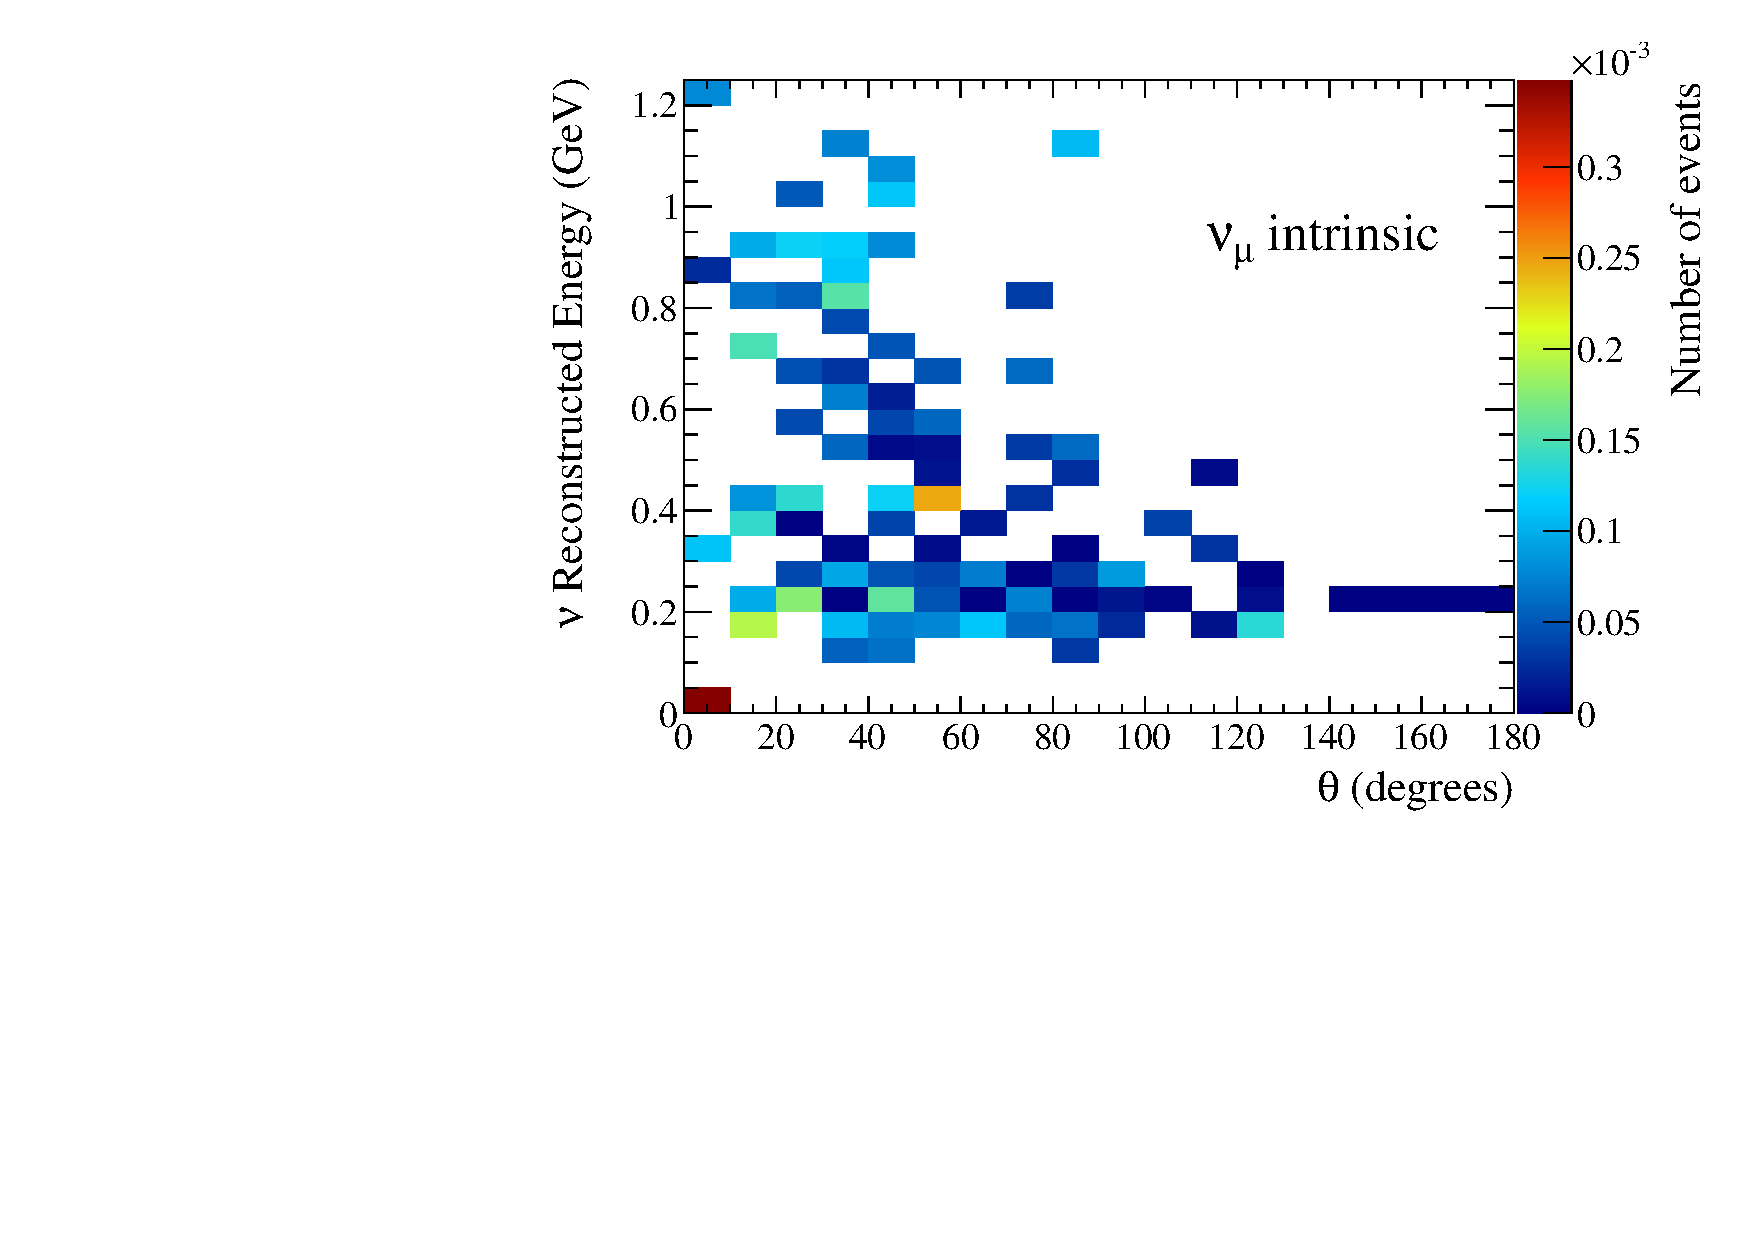
\includegraphics[width=0.9\textwidth]{joint_plots/spectrum_predictions/template_ereco_vs_theta_numubeam_rhc1re.pdf}
\caption{$\nu_{\mu}$ intrinsic beam.}
\end{subfigure}
\begin{subfigure}[b]{0.49\textwidth}
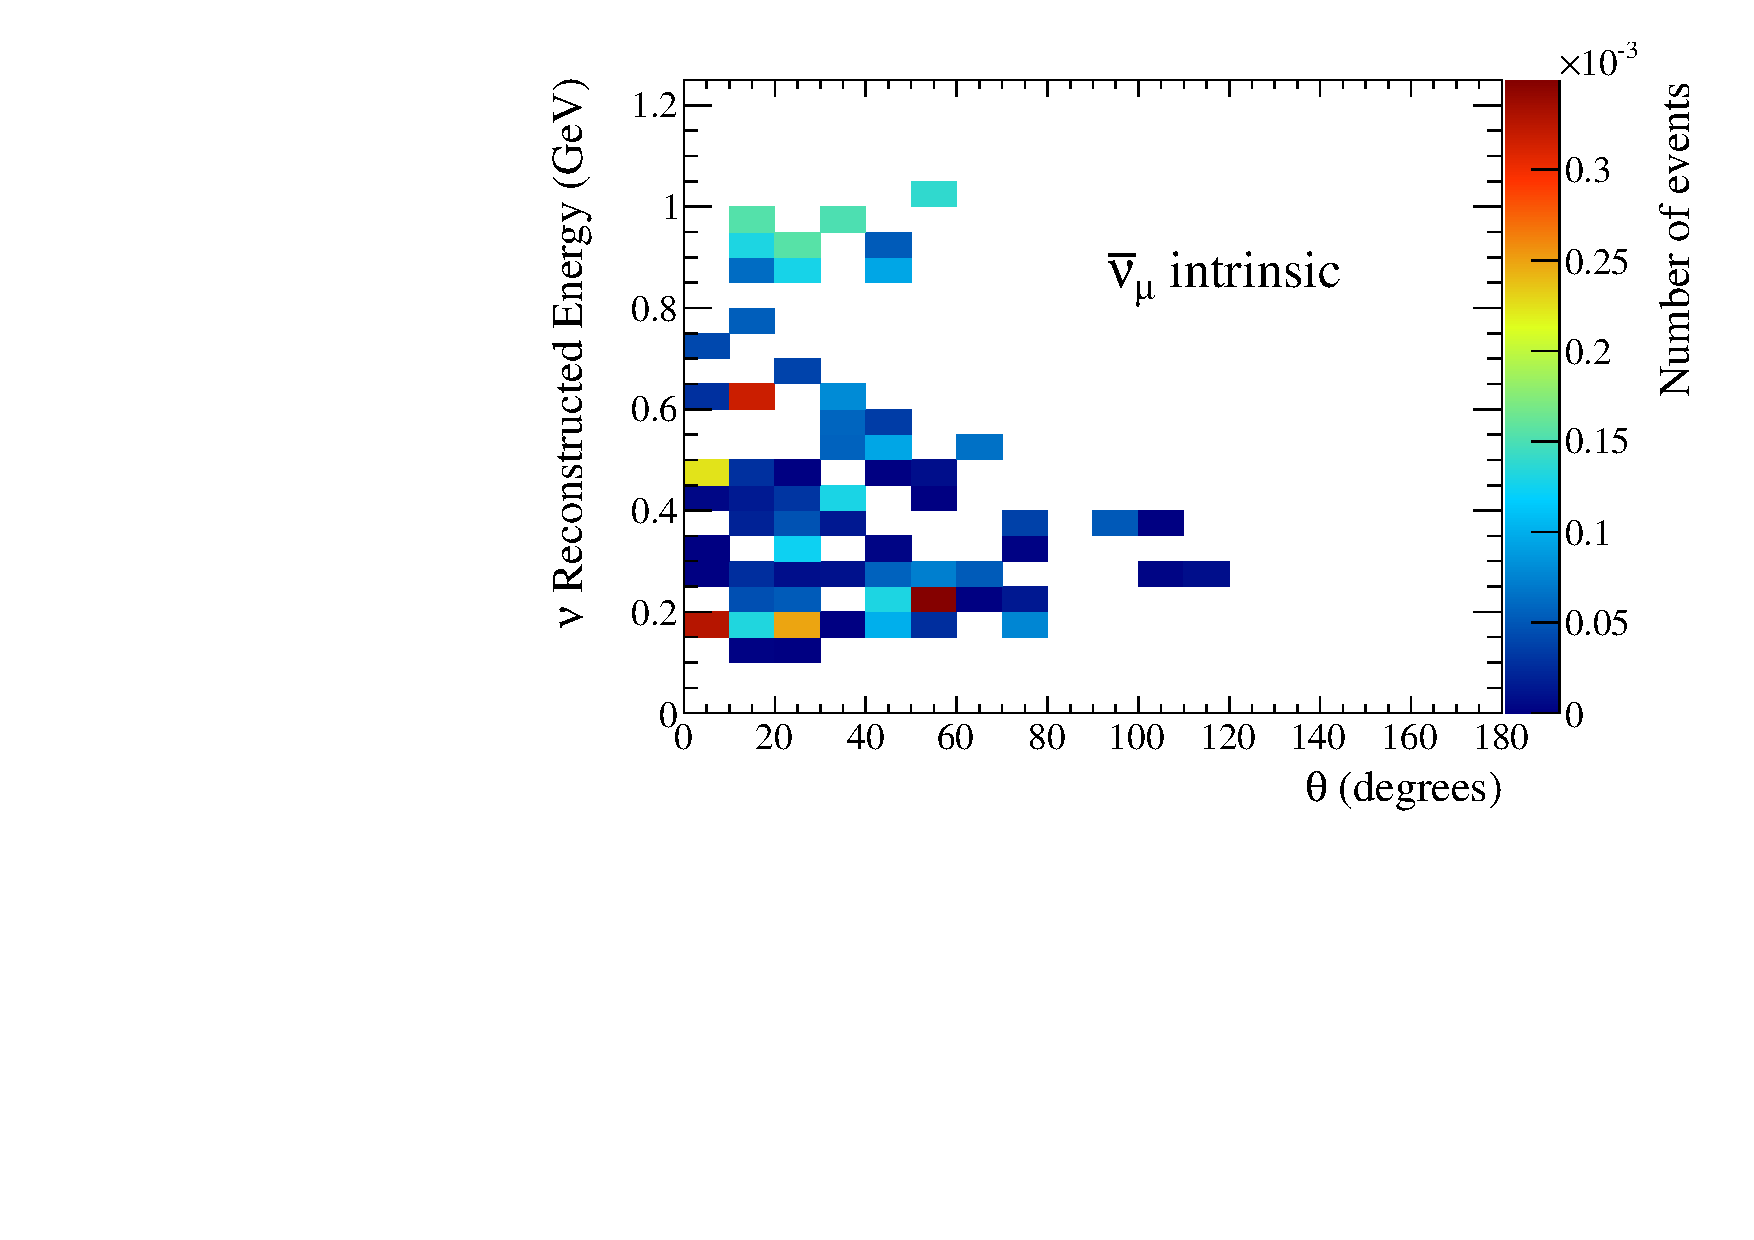
\includegraphics[width=0.9\textwidth]{joint_plots/spectrum_predictions/template_ereco_vs_theta_numubarbeam_rhc1re.pdf}
\caption{$\bar{\nu}_{\mu}$ intrinsic beam.}
\end{subfigure}
\caption {
Predicted spectra of electron-like events
as a function of the reconstructed neutrino energy and
the angle between the outgoing lepton and the neutrino direction.
The distributions correspond to the collected statistics in the full Run 1-6 data set
for an exposure.
%of $6.914 \times 10^{20}$ POT in neutrino  mode.
%and
%of $4.011 \times 10^{20}$ POT in antineutrino mode.
From top left to bottom right the following components are shown:
total,
$\nu_{\mu} \rightarrow \nu_e$,
$\bar{\nu}_{\mu} \rightarrow \bar{\nu}_e$,
$\nu_e + \bar{\nu}_e$ intrinsic beam,
NC,
$\nu_{\mu}$ intrinsic beam
and
$\bar{\nu}_{\mu}$ intrinsic beam.
The spectra were generated with the systematic parameters measured with the ND280 data 
shown in \cref{tab:banff_uncertainties_flux_fhc},~\ref{tab:banff_uncertainties_flux_rhc},~\ref{tab:banff_uncertainties_xsec},
the nominal Super-K systematic parameters shown in \cref{tab:banff_uncertainties_skdetfsi}
and the oscillation parameters corresponding to the Asimov data set A shown in \cref{tab:osc_params_joint_asimov}.
}
\label{fig:joint_ereco_vs_theta_rhc1re}
\end{figure*}


In \cref{fig:joint_1d_elike} the projection of the 2-dimensional $e$-like templates
onto the $E_{reco}$ and $\theta$ axes are shown.

\begin{figure*}[htb]
%\hspace{0.06\linewidth}
\center
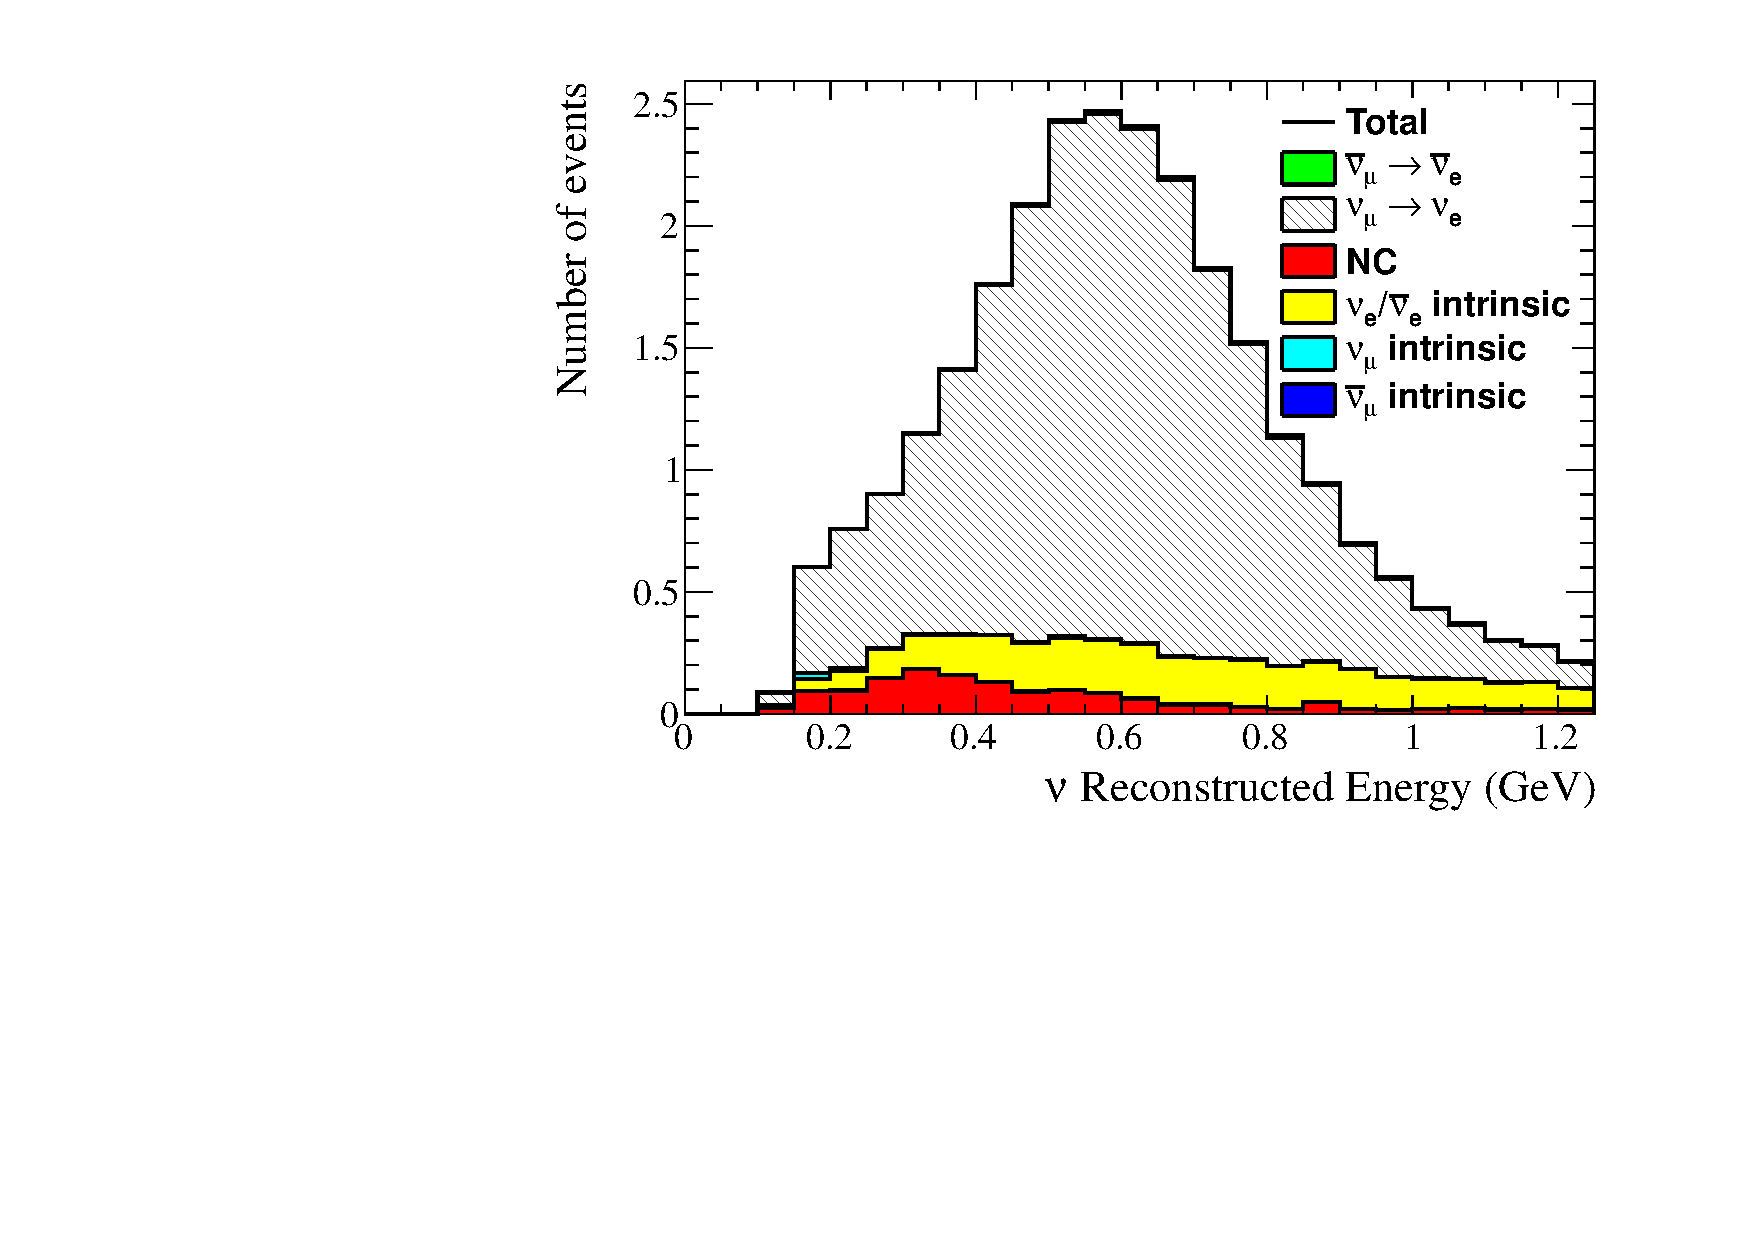
\includegraphics[width=18pc]{joint_plots/spectrum_predictions/template_ereco_1re.pdf}
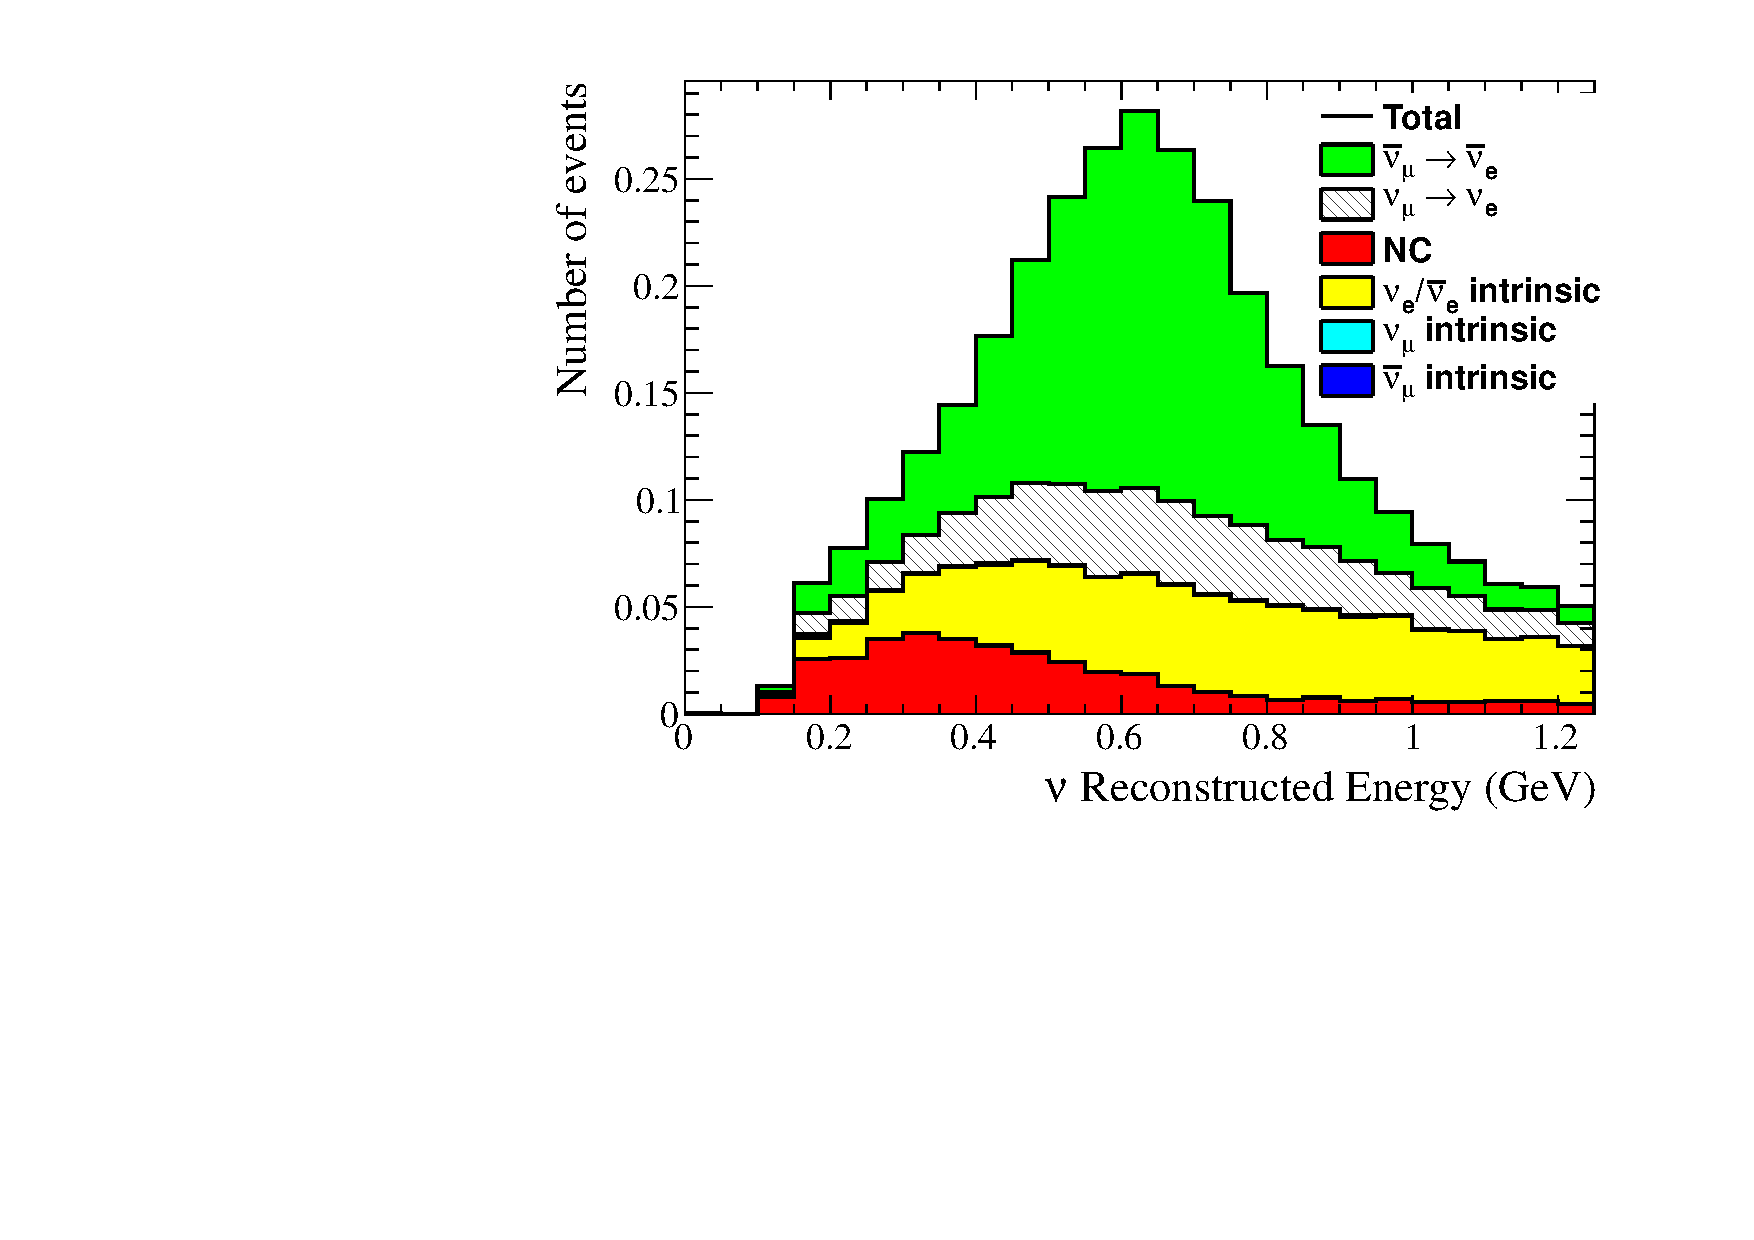
\includegraphics[width=18pc]{joint_plots/spectrum_predictions/template_ereco_rhc1re.pdf}
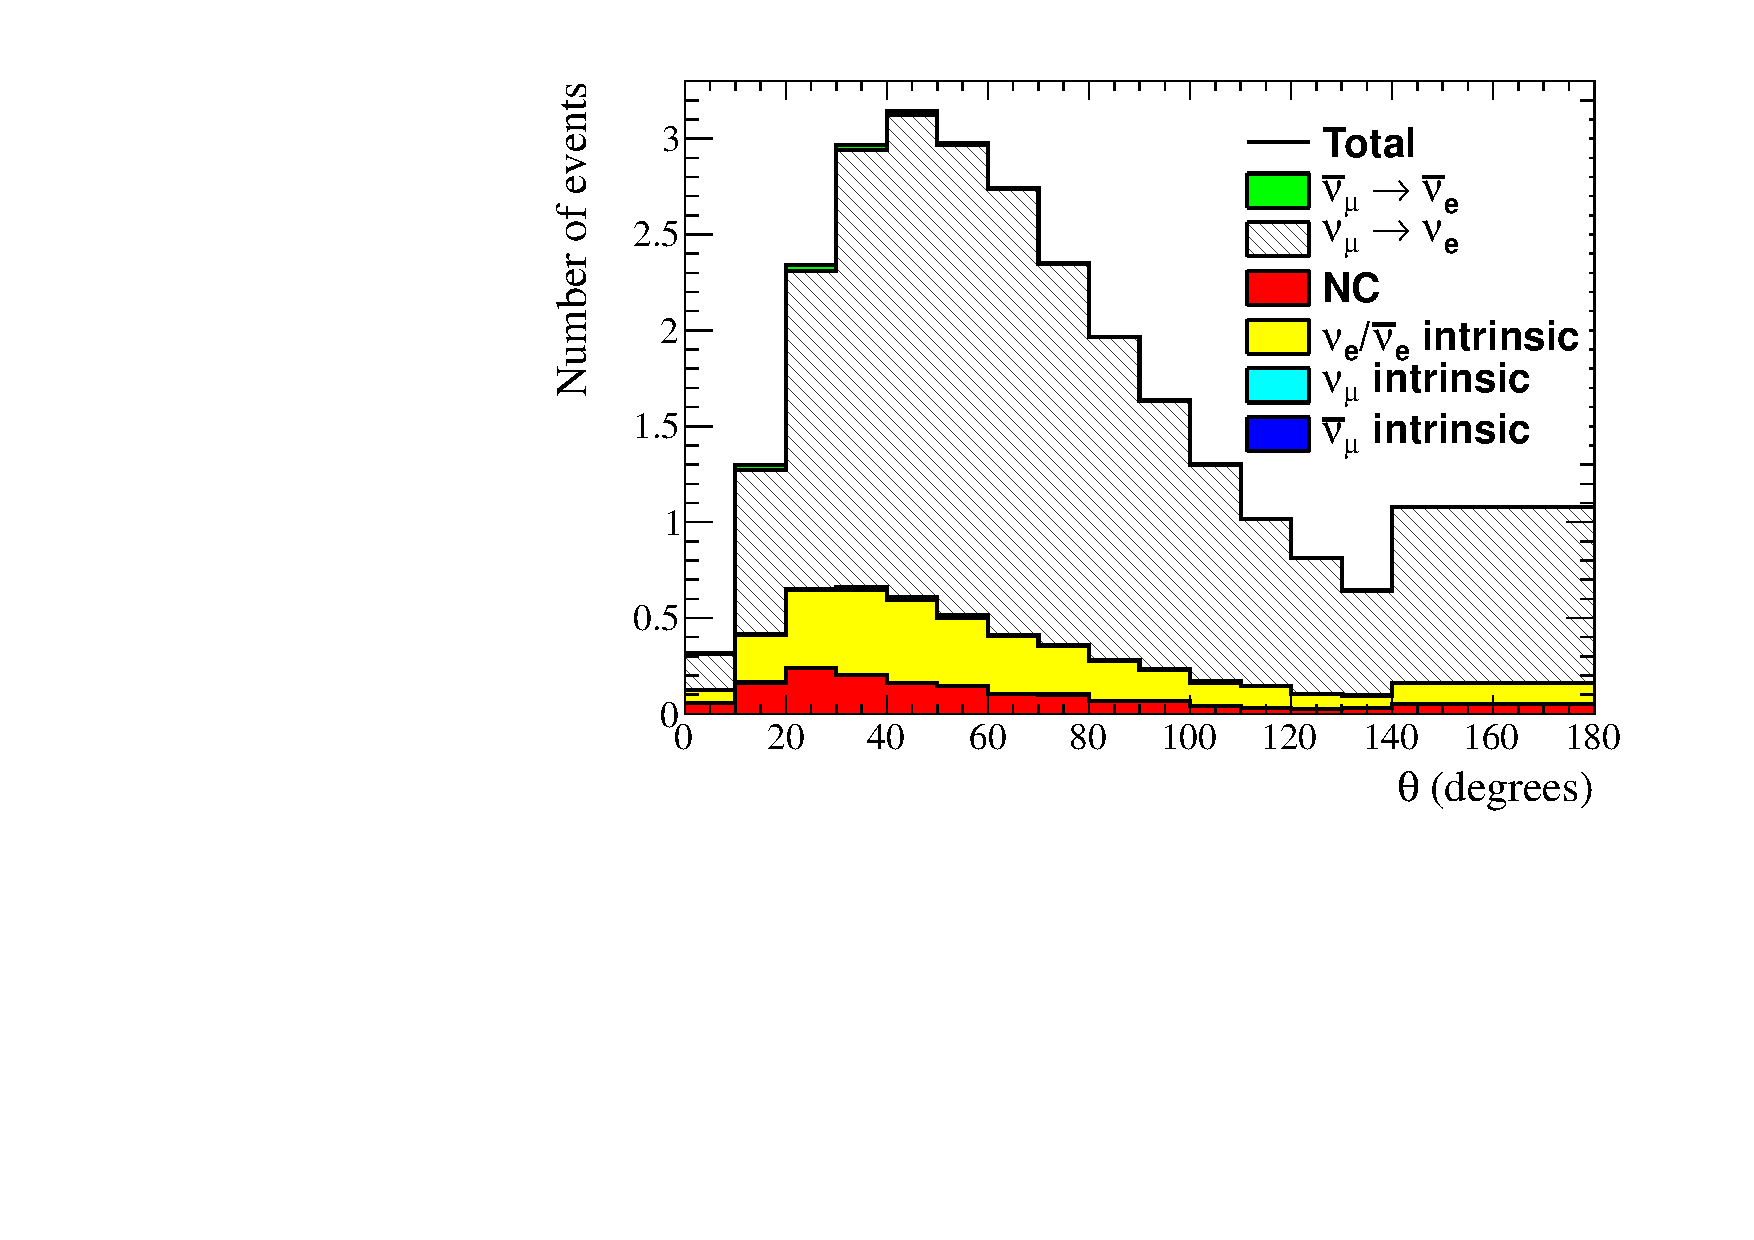
\includegraphics[width=18pc]{joint_plots/spectrum_predictions/template_theta_1re.pdf}
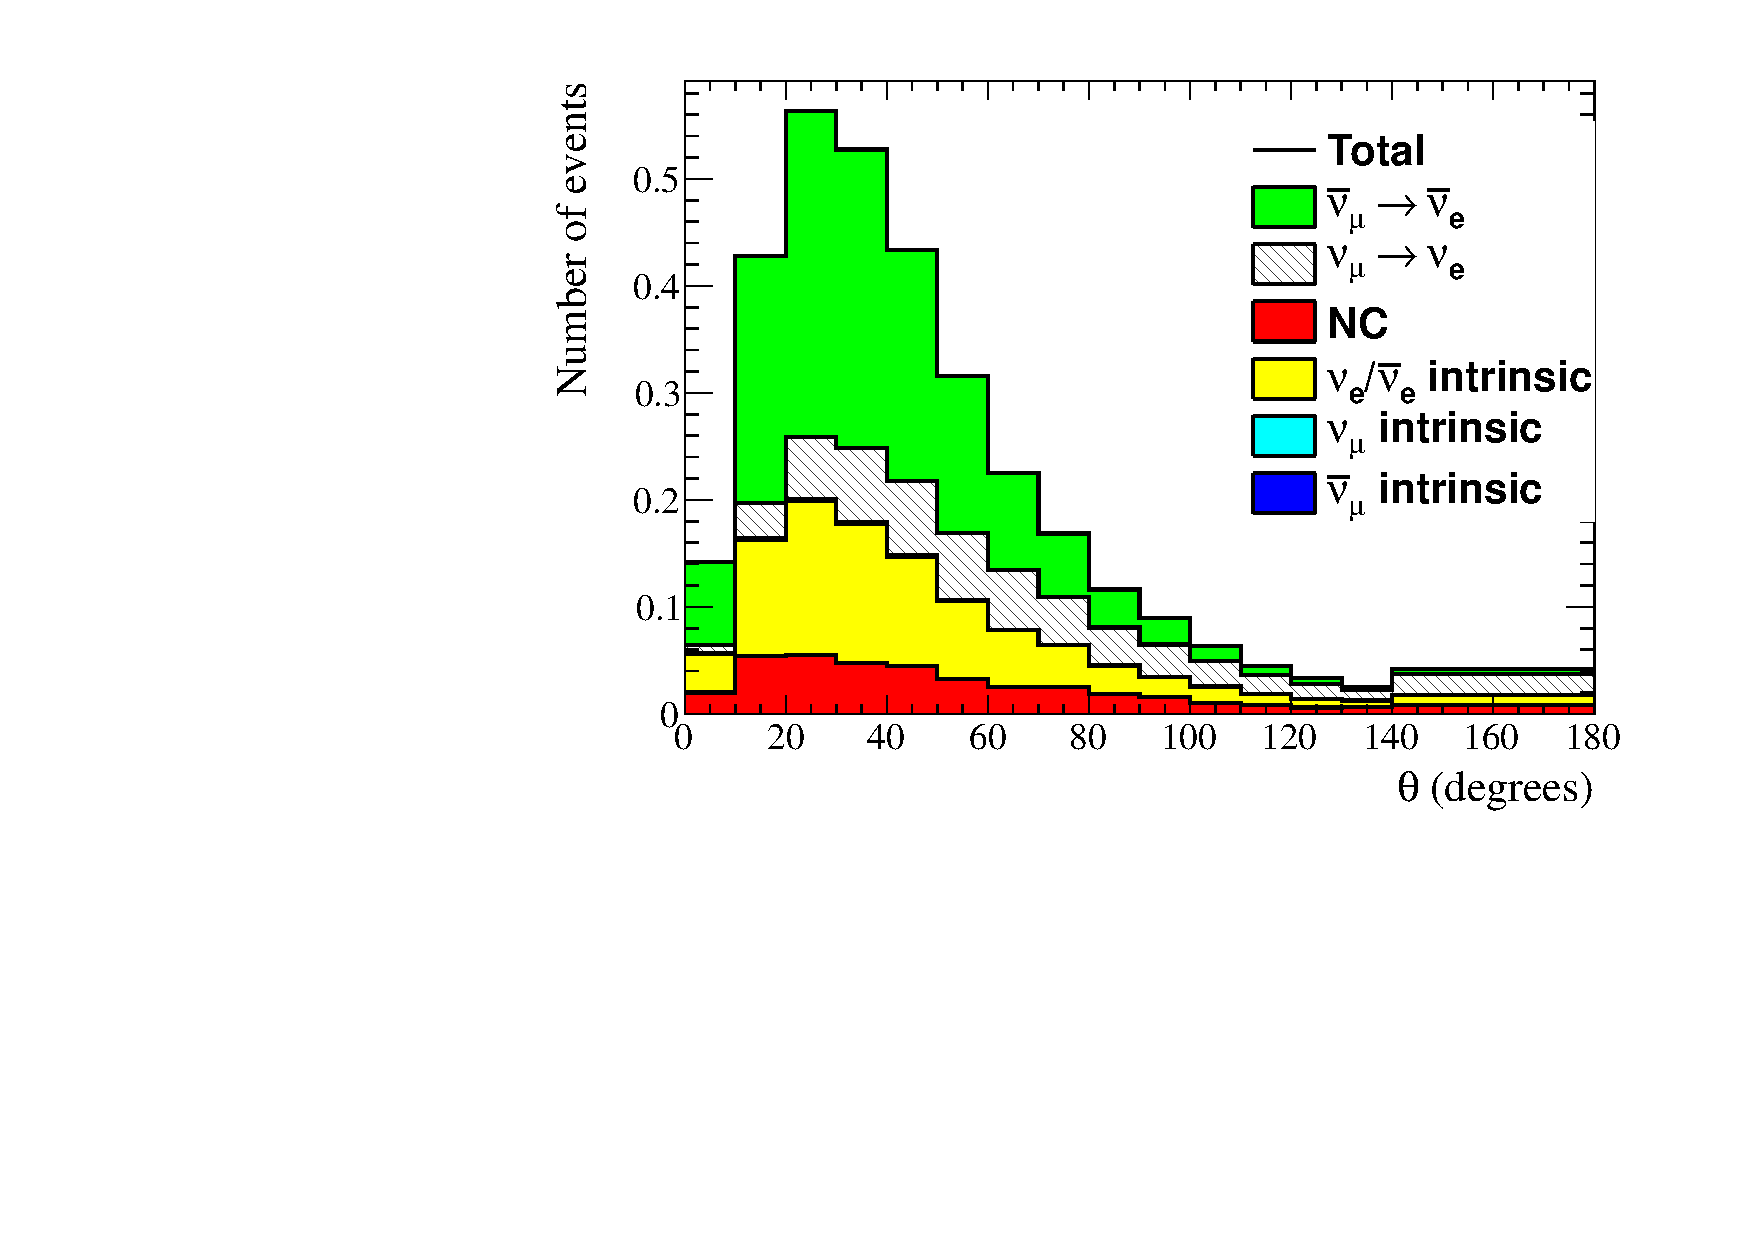
\includegraphics[width=18pc]{joint_plots/spectrum_predictions/template_theta_rhc1re.pdf}
\caption {
Predicted spectra of 
the reconstructed neutrino energy (top) 
and
the angle between the neutrino and the outgoing lepton directions (bottom)
for electron-like 
neutrino mode (left)
and
antineutrino mode (right)
events.
The distributions correspond to the collected statistics in the full Run 1-6 data set.
%for an exposure 
%of $6.914 \times 10^{20}$ POT in neutrino mode
%and
%of $4.011 \times 10^{20}$ POT in antineutrino mode.
The distributions are broken down by the following components:
$\bar{\nu}_{\mu} \to \bar{\nu}_e$ (green), 
$\nu_{\mu} \to \nu_e$ (black/white), 
NC (red),
$\nu_e + \bar{\nu}_e$ intrinsic beam (yellow),
$\nu_{\mu}$ intrinsic beam (light blue)
and
$\bar{\nu}_{\mu}$ intrinsic beam (blue).
The spectra were generated with the systematic parameters measured with the ND280 data 
shown in \cref{tab:banff_uncertainties_flux_fhc},~\ref{tab:banff_uncertainties_flux_rhc},~\ref{tab:banff_uncertainties_xsec},
the nominal Super-K systematic parameters shown in \cref{tab:banff_uncertainties_skdetfsi}
and the oscillation parameters corresponding to the Asimov data set A shown in \cref{tab:osc_params_joint_asimov}.
}
\label{fig:joint_1d_elike}
\end{figure*}


%\clearpage


\clearpage


%...........................................................
%
% Observed spectra
%
%...........................................................

\section{Observed $e$-like spectra}
\label{app:templates_observed}

In \cref{fig:joint_ereco_vs_theta_1re_data} and~\ref{fig:joint_ereco_vs_theta_rhc1re_data}
the predicted breakdown of the $e$-like 2-dimensional spectra are compared to data for
both neutrino and antineutrino beam mode.

\begin{figure*}[htb]
\center
\begin{subfigure}[b]{0.49\textwidth}
\includegraphics[width=0.9\textwidth]{./joint_plots/data/data_mc_1re_2d_NuMuToNue.pdf}
\caption{$\nu_{\mu} \rightarrow \nu_e$.}
\end{subfigure}
\begin{subfigure}[b]{0.49\textwidth}
\includegraphics[width=0.9\textwidth]{./joint_plots/data/data_mc_1re_2d_NuMuBarToNueBar.pdf}
\caption{$\bar{\nu}_{\mu} \rightarrow \bar{\nu}_e$.}
\end{subfigure}
\begin{subfigure}[b]{0.49\textwidth}
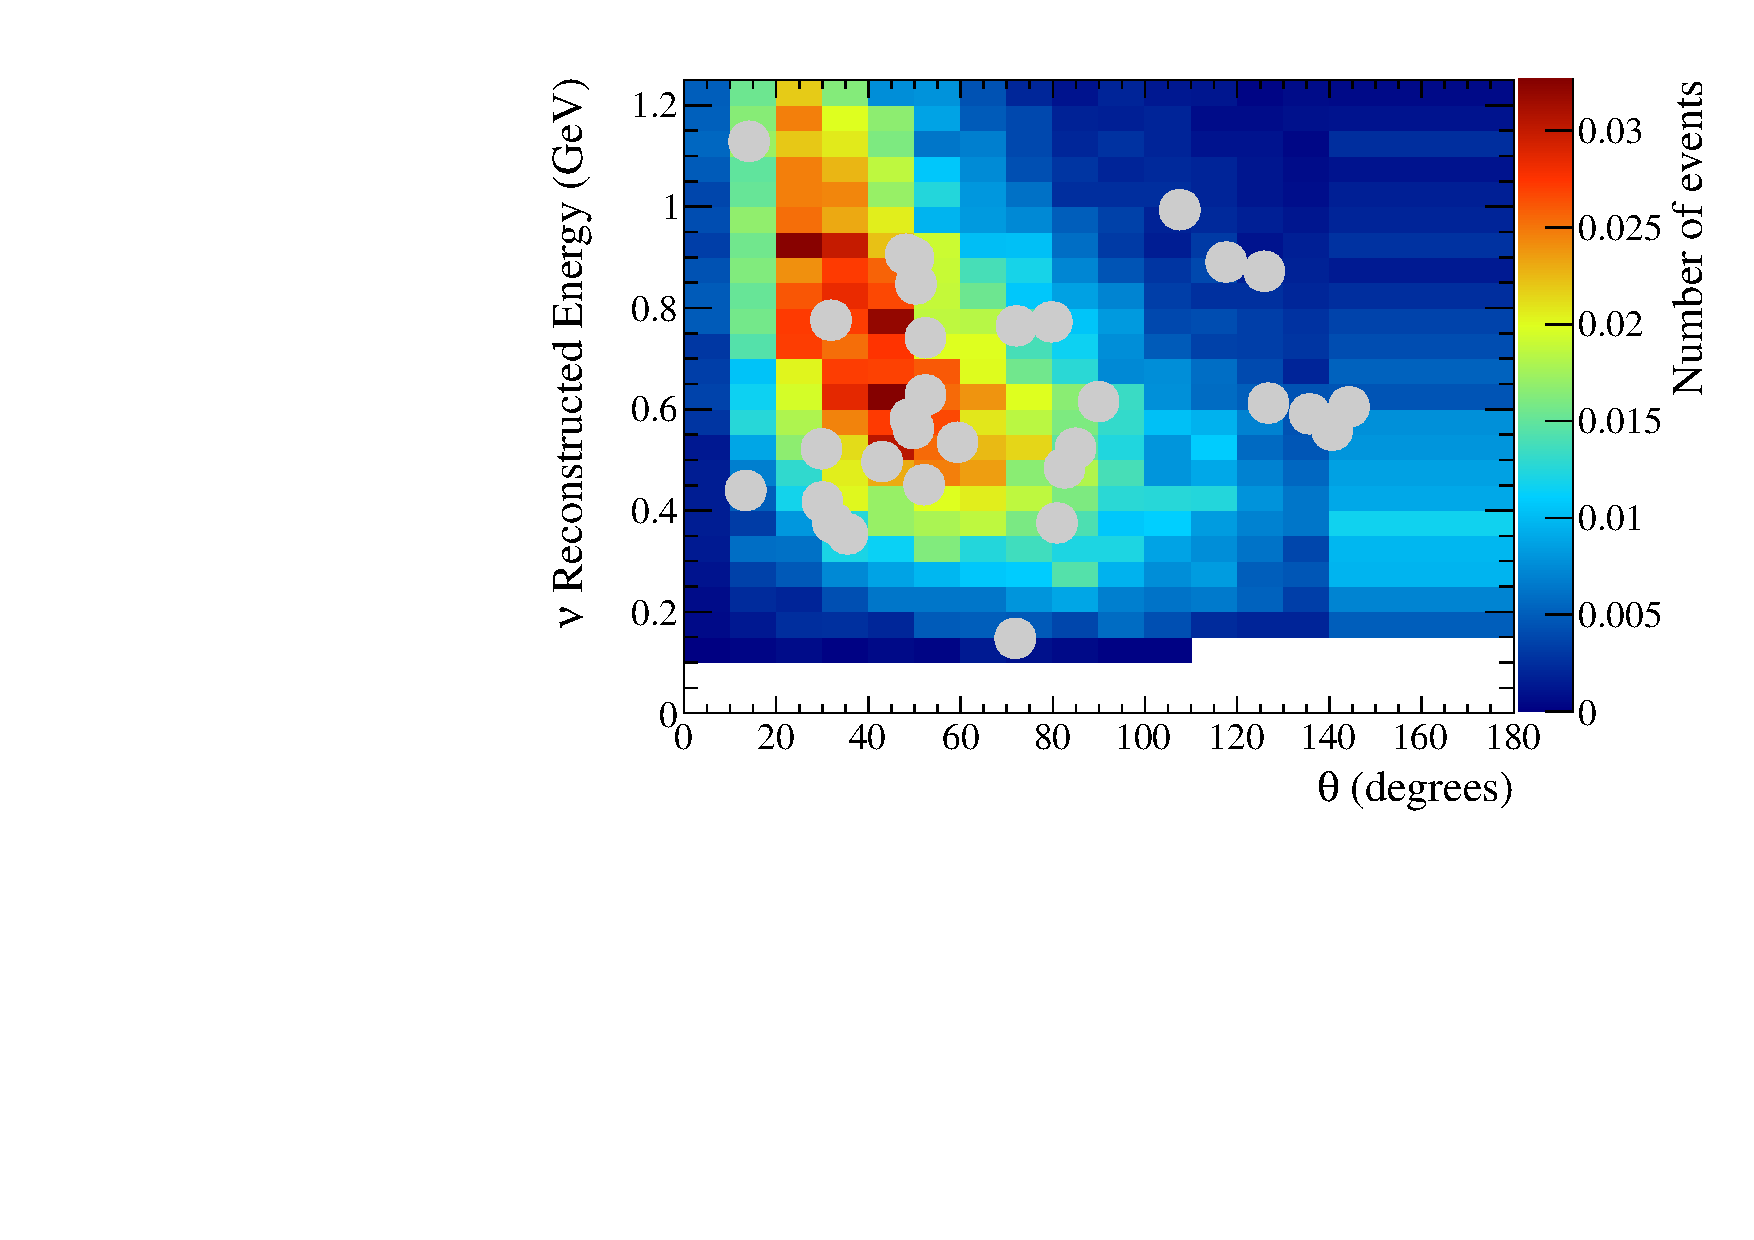
\includegraphics[width=0.9\textwidth]{./joint_plots/data/data_mc_1re_2d_NueBeam.pdf}
\caption{$\nu_{e}$ + $\bar{\nu}_e$ intrinsic beam.}
\end{subfigure}
\begin{subfigure}[b]{0.49\textwidth}
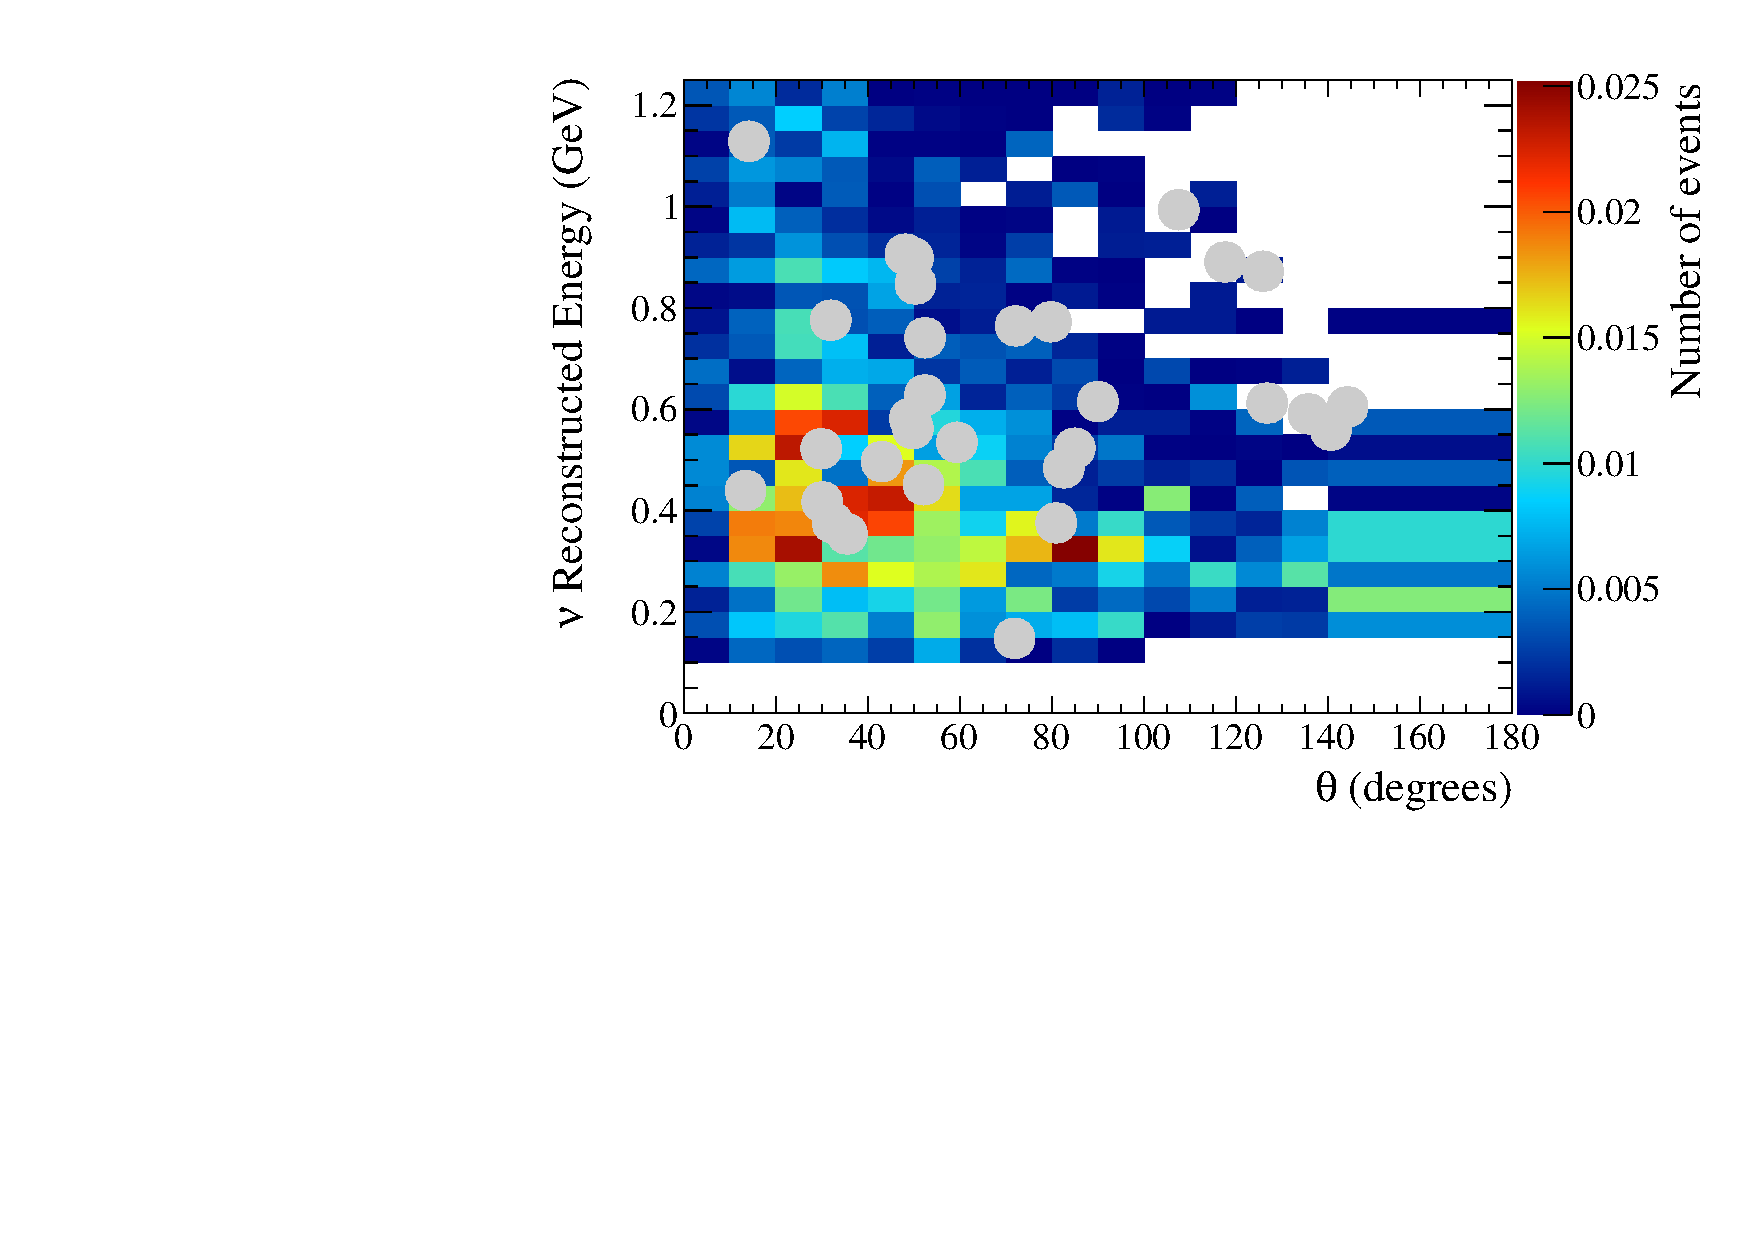
\includegraphics[width=0.9\textwidth]{./joint_plots/data/data_mc_1re_2d_NC.pdf}
\caption{Neutral current.}
\end{subfigure}
\begin{subfigure}[b]{0.49\textwidth}
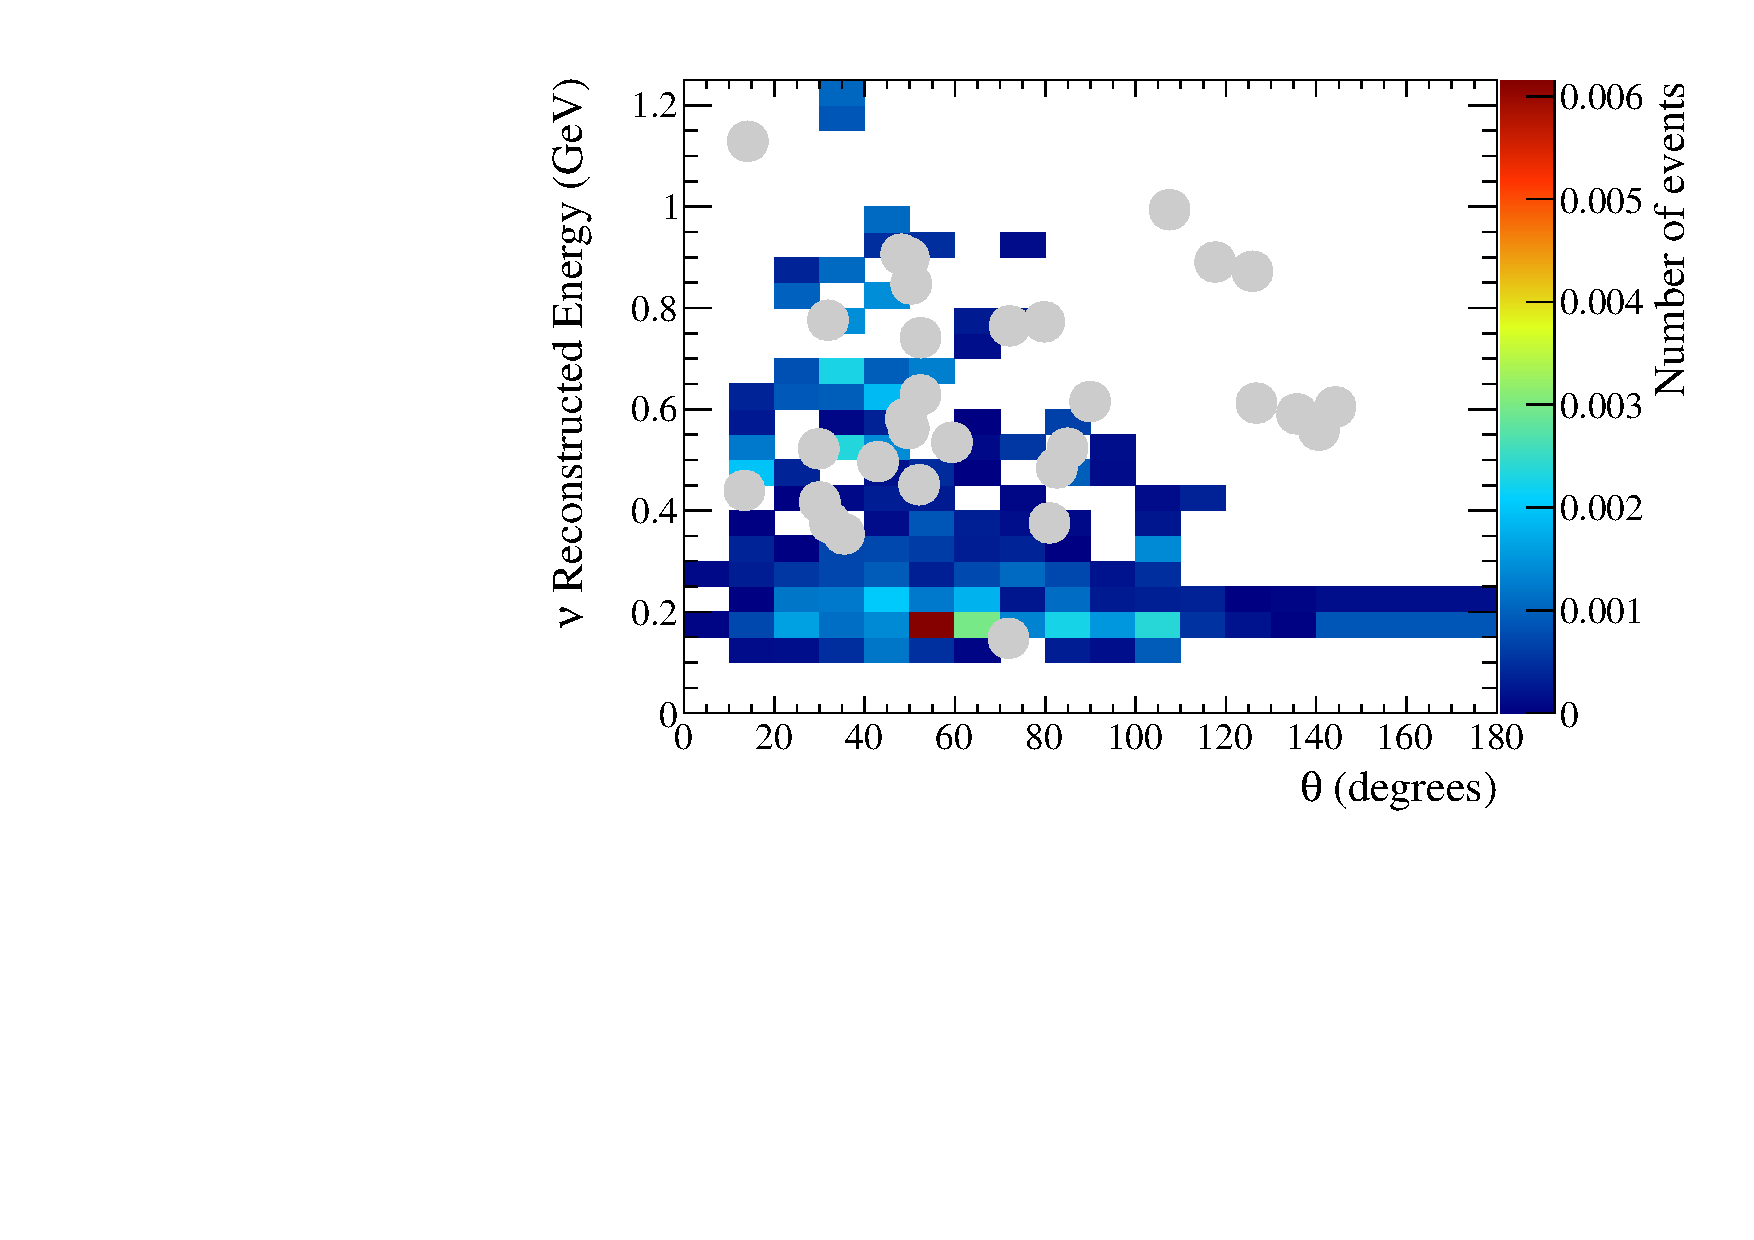
\includegraphics[width=0.9\textwidth]{./joint_plots/data/data_mc_1re_2d_NumuBeam.pdf}
\caption{$\nu_{\mu}$ intrinsic beam.}
\end{subfigure}
\begin{subfigure}[b]{0.49\textwidth}
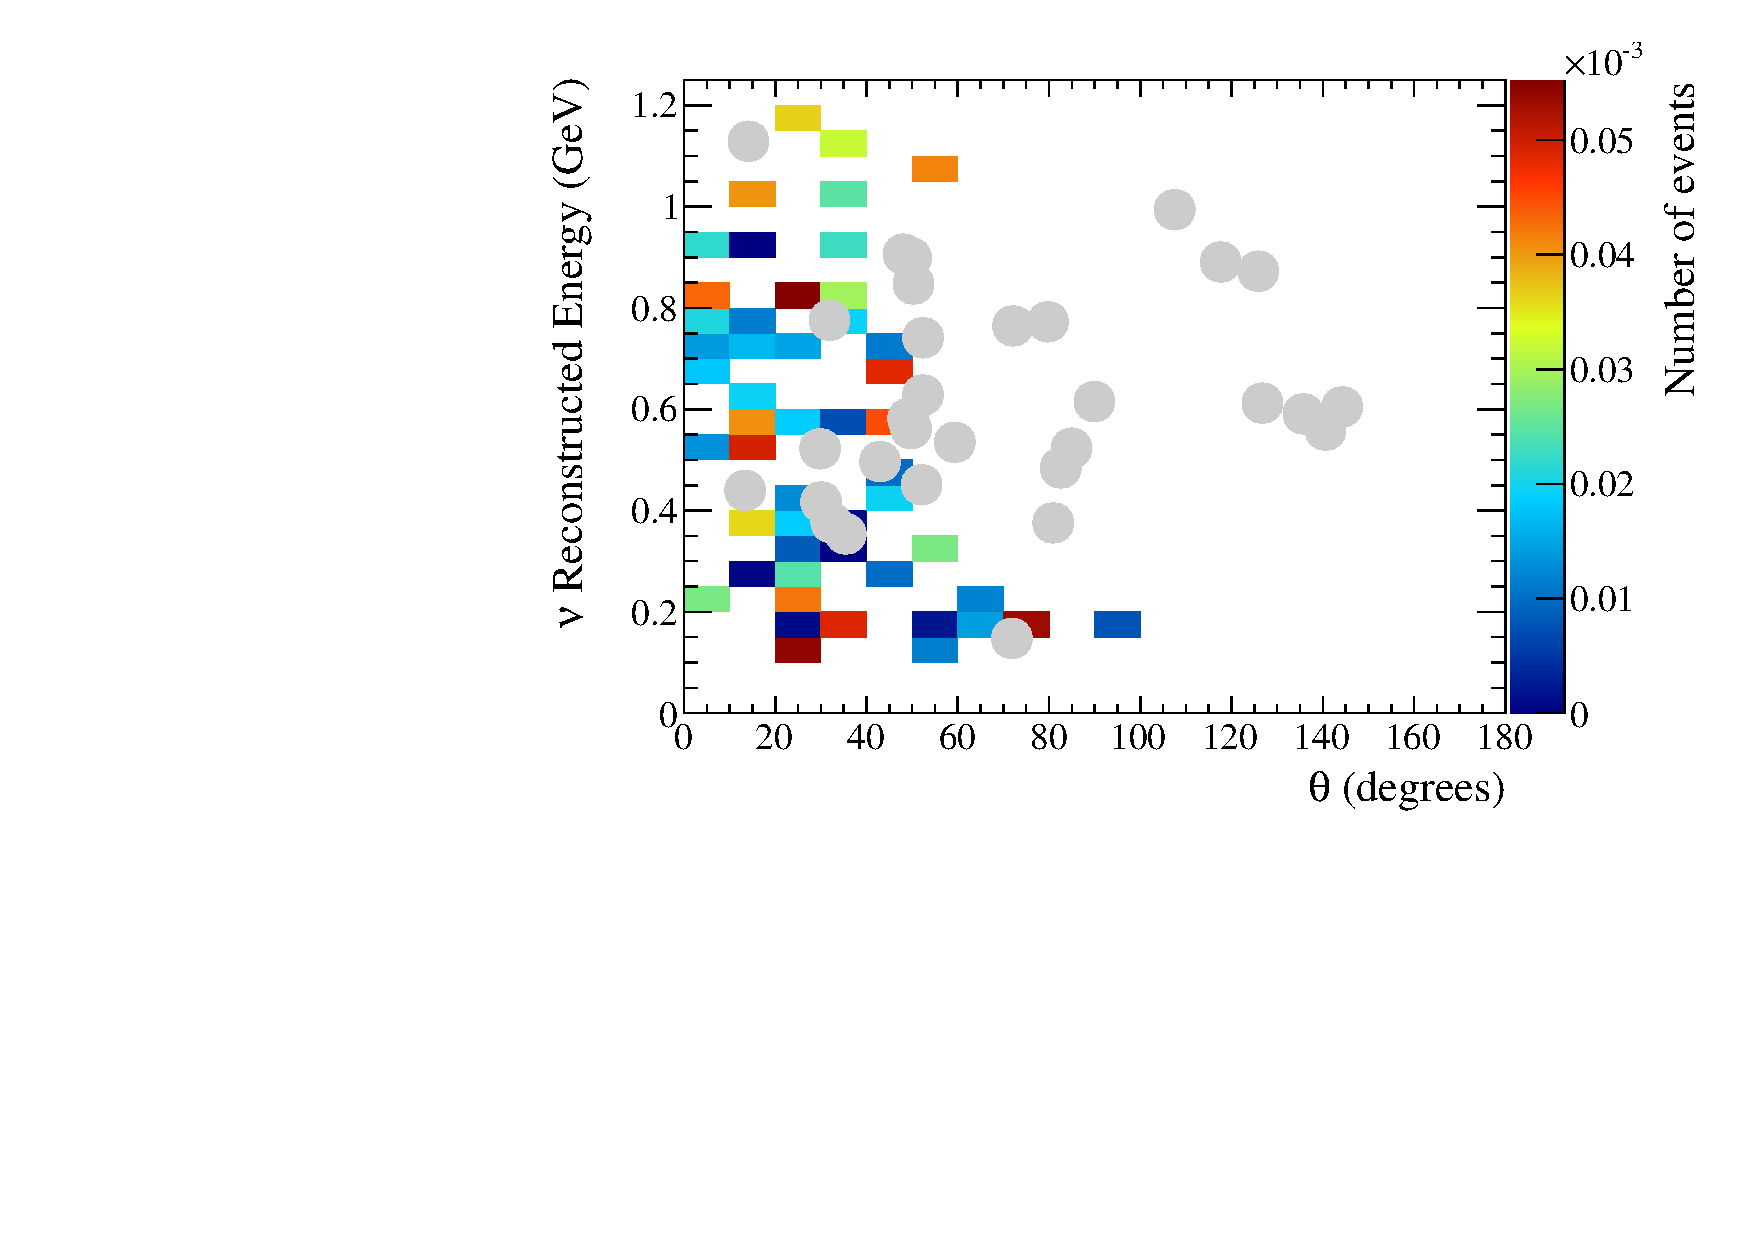
\includegraphics[width=0.9\textwidth]{./joint_plots/data/data_mc_1re_2d_NumuBarBeam.pdf}
\caption{$\bar{\nu}_{\mu}$ intrinsic beam.}
\end{subfigure}
\caption {
Predicted and observed (grey dots) spectra of electron-like events
as a function of the reconstructed neutrino energy and
the angle between the outgoing lepton and the neutrino direction.
The distributions correspond to the collected statistics in the full Run 1-6 data set.
%for an exposure 
%of $6.914 \times 10^{20}$ POT in neutrino mode.
%and
%of $4.011 \times 10^{20}$ POT in antineutrino mode.
From top left to bottom right the following components are shown:
%total,
$\nu_{\mu} \rightarrow \nu_e$,
$\bar{\nu}_{\mu} \rightarrow \bar{\nu}_e$,
$\nu_e + \bar{\nu}_e$ intrinsic beam,
NC,
$\nu_{\mu}$ intrinsic beam
and
$\bar{\nu}_{\mu}$ intrinsic beam.
The spectra were generated with the systematic parameters measured with the ND280 data 
shown in \cref{tab:banff_uncertainties_flux_fhc},~\ref{tab:banff_uncertainties_flux_rhc},~\ref{tab:banff_uncertainties_xsec},
the nominal Super-K systematic parameters shown in \cref{tab:banff_uncertainties_skdetfsi}
and the oscillation parameters corresponding to the Asimov data set A shown in \cref{tab:osc_params_joint_asimov}.
}
\label{fig:joint_ereco_vs_theta_1re_data}
\end{figure*}

\begin{figure*}[htb]
\center
\begin{subfigure}[b]{0.49\textwidth}
\includegraphics[width=0.9\textwidth]{./joint_plots/data/data_mc_rhc1re_2d_NuMuToNue.pdf}
\caption{$\nu_{\mu} \rightarrow \nu_e$.}
\end{subfigure}
\begin{subfigure}[b]{0.49\textwidth}
\includegraphics[width=0.9\textwidth]{./joint_plots/data/data_mc_rhc1re_2d_NuMuBarToNueBar.pdf}
\caption{$\bar{\nu}_{\mu} \rightarrow \bar{\nu}_e$.}
\end{subfigure}
\begin{subfigure}[b]{0.49\textwidth}
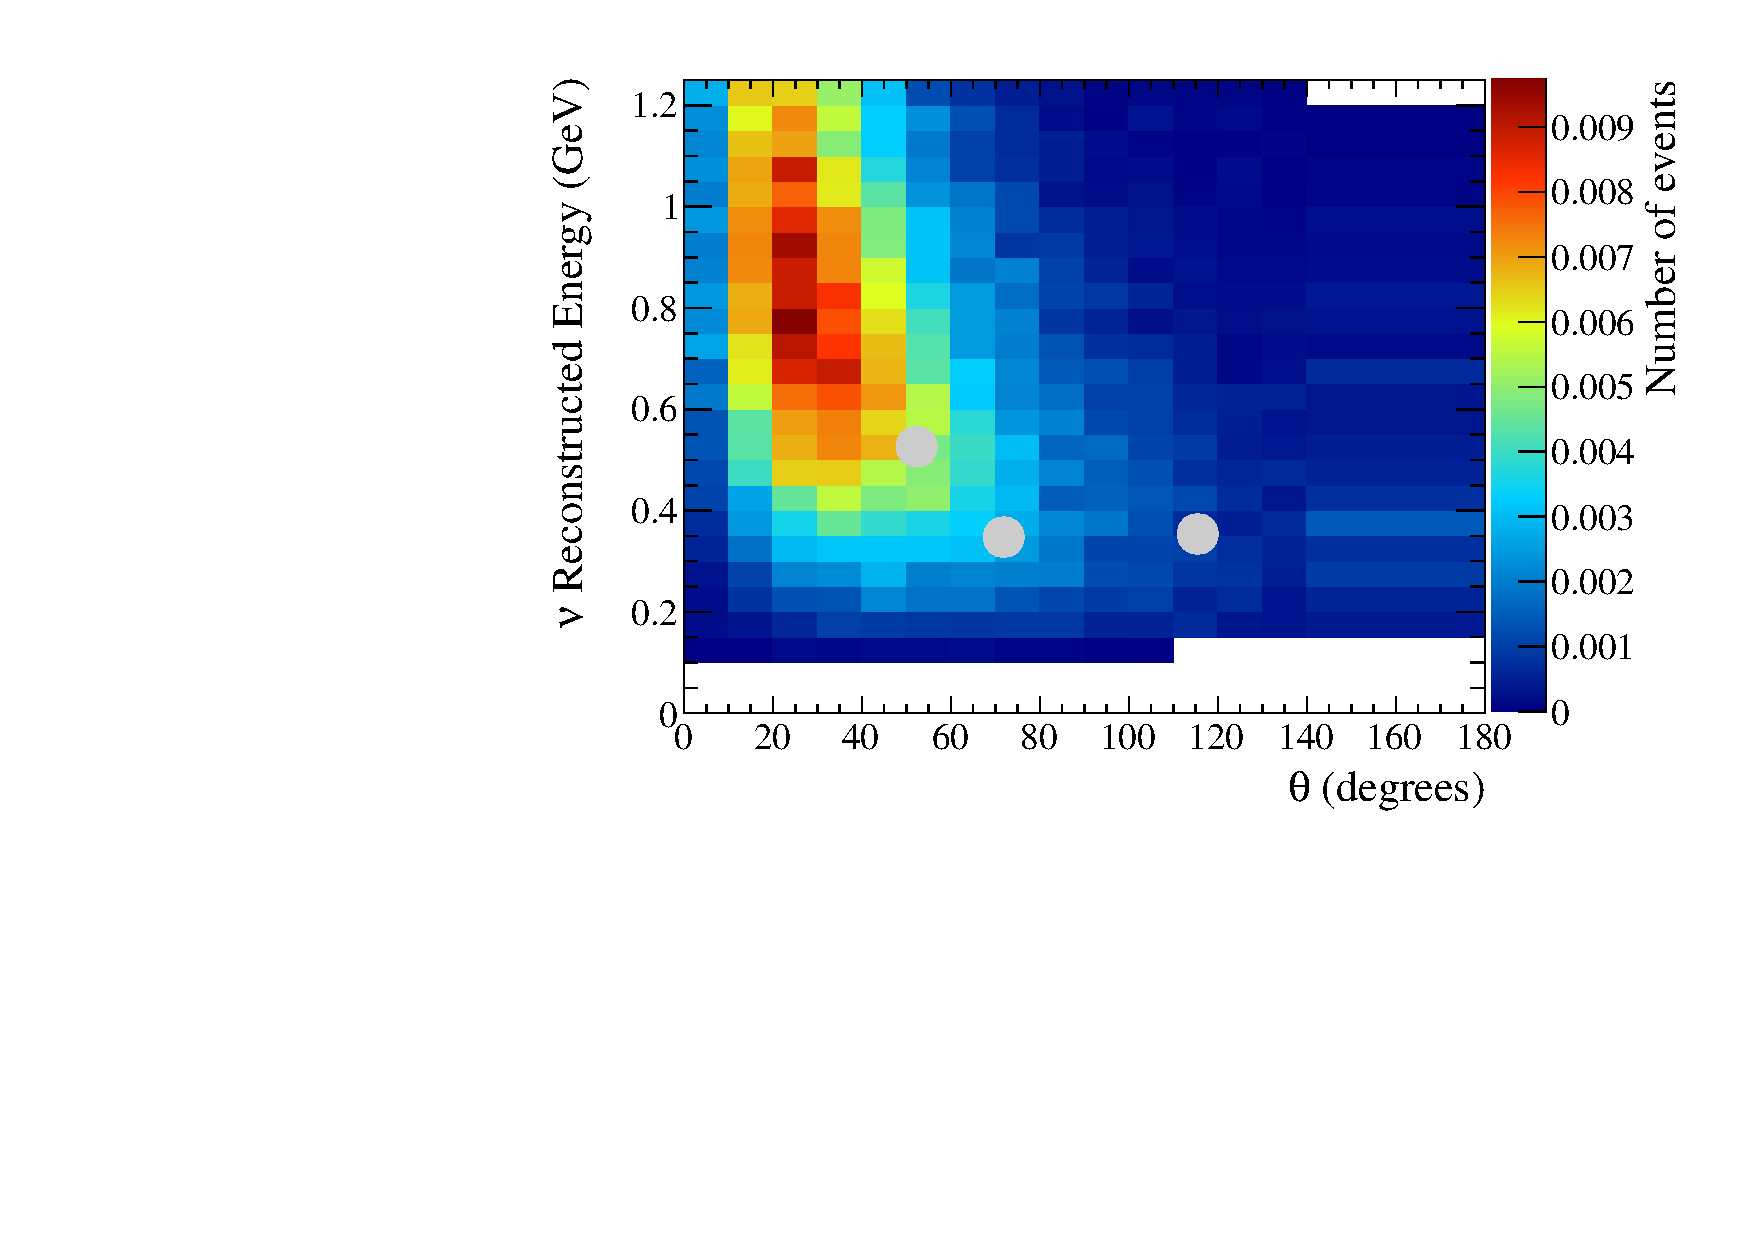
\includegraphics[width=0.9\textwidth]{./joint_plots/data/data_mc_rhc1re_2d_NueBeam.pdf}
\caption{$\nu_{e}$ + $\bar{\nu}_e$ intrinsic beam.}
\end{subfigure}
\begin{subfigure}[b]{0.49\textwidth}
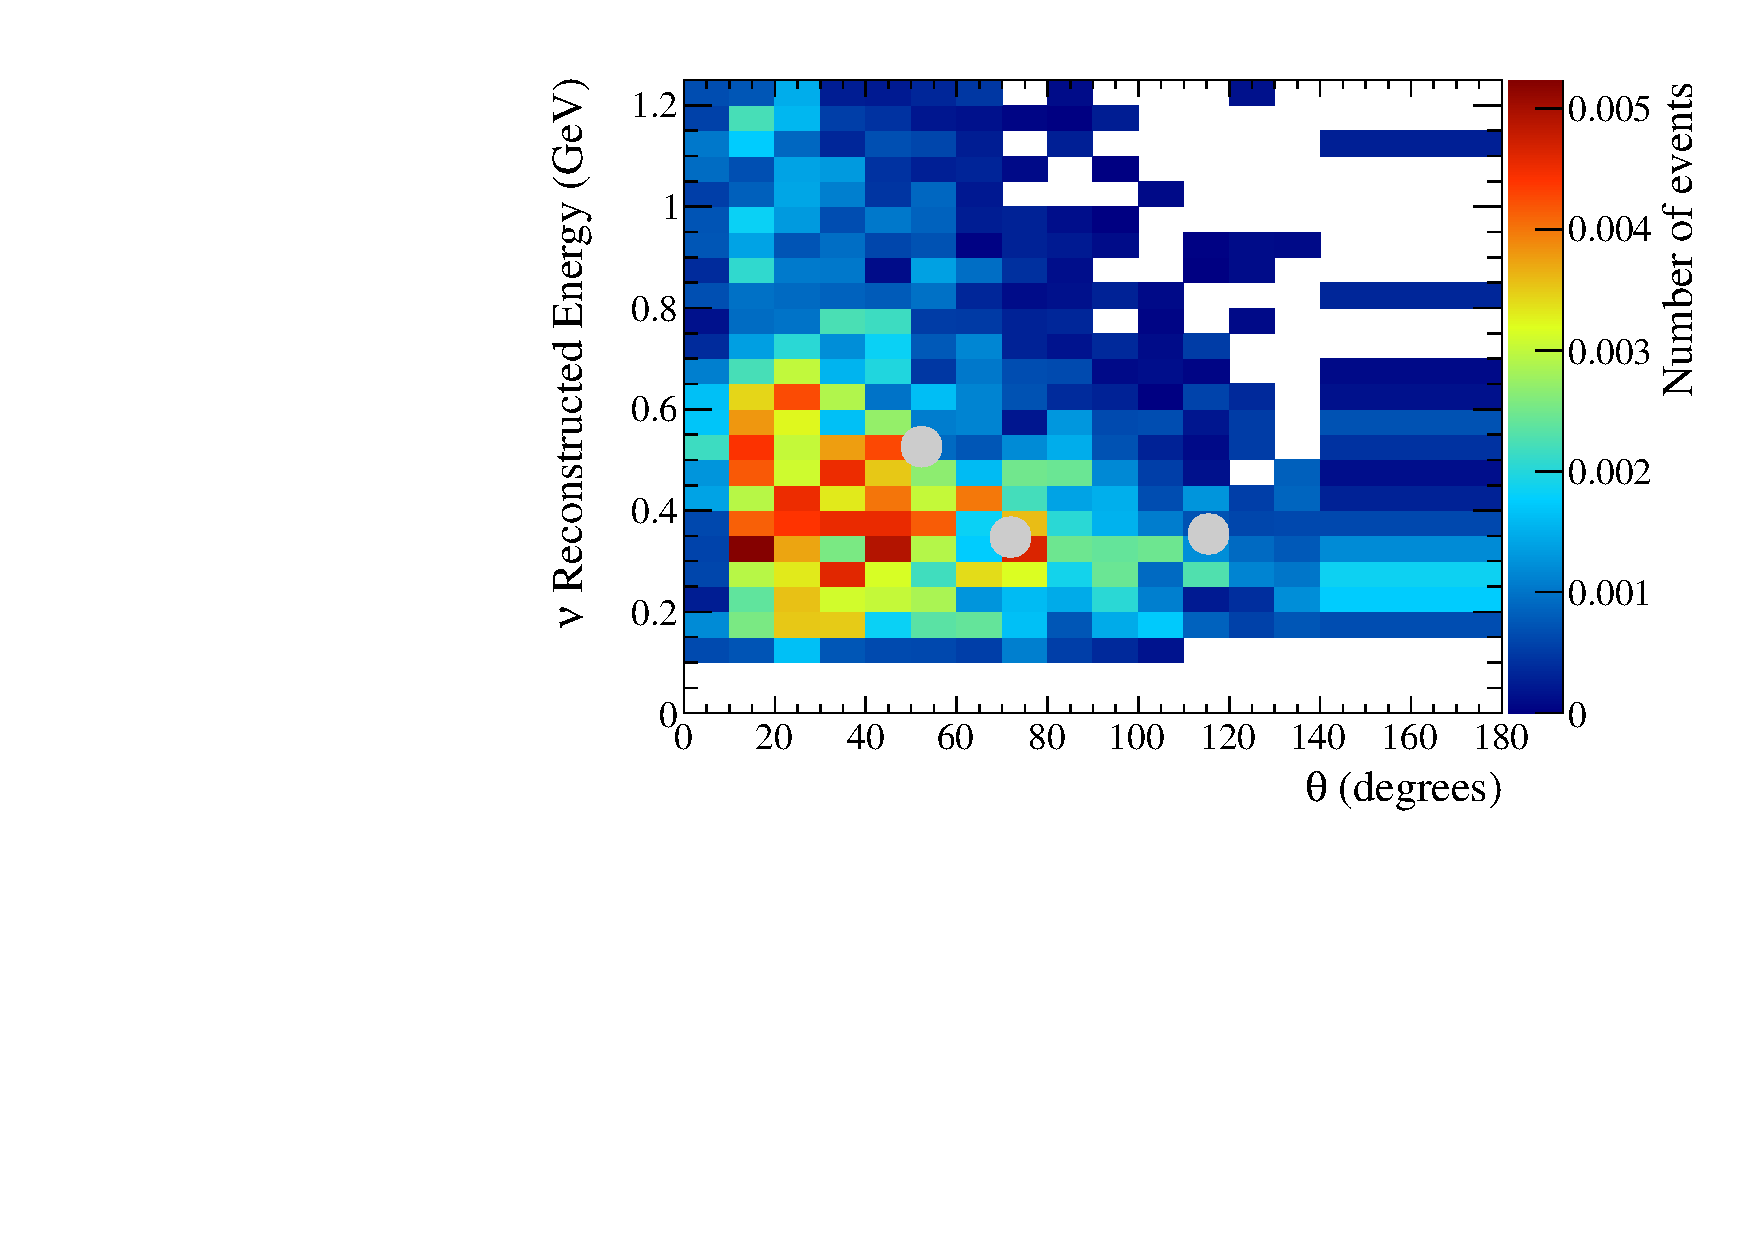
\includegraphics[width=0.9\textwidth]{./joint_plots/data/data_mc_rhc1re_2d_NC.pdf}
\caption{Neutral current.}
\end{subfigure}
\begin{subfigure}[b]{0.49\textwidth}
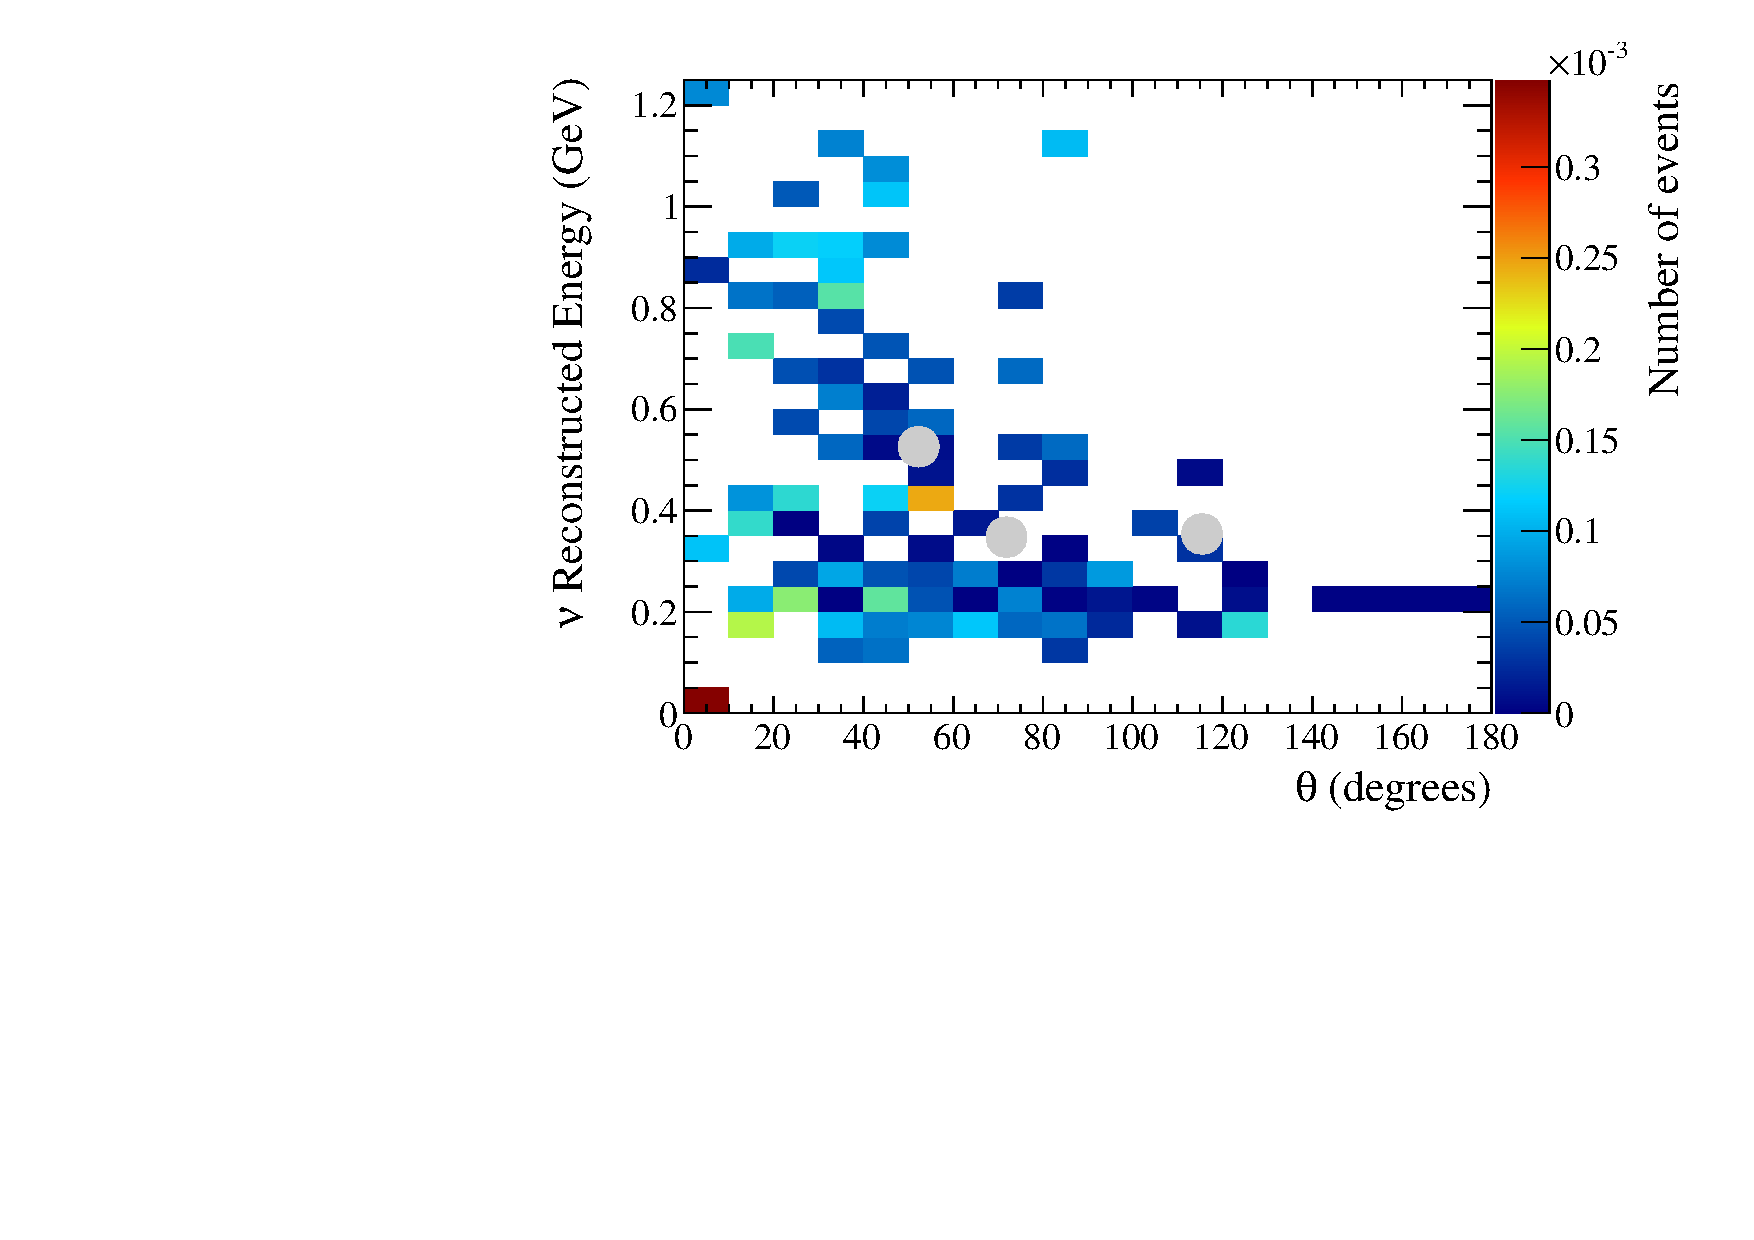
\includegraphics[width=0.9\textwidth]{./joint_plots/data/data_mc_rhc1re_2d_NumuBeam.pdf}
\caption{$\nu_{\mu}$ intrinsic beam.}
\end{subfigure}
\begin{subfigure}[b]{0.49\textwidth}
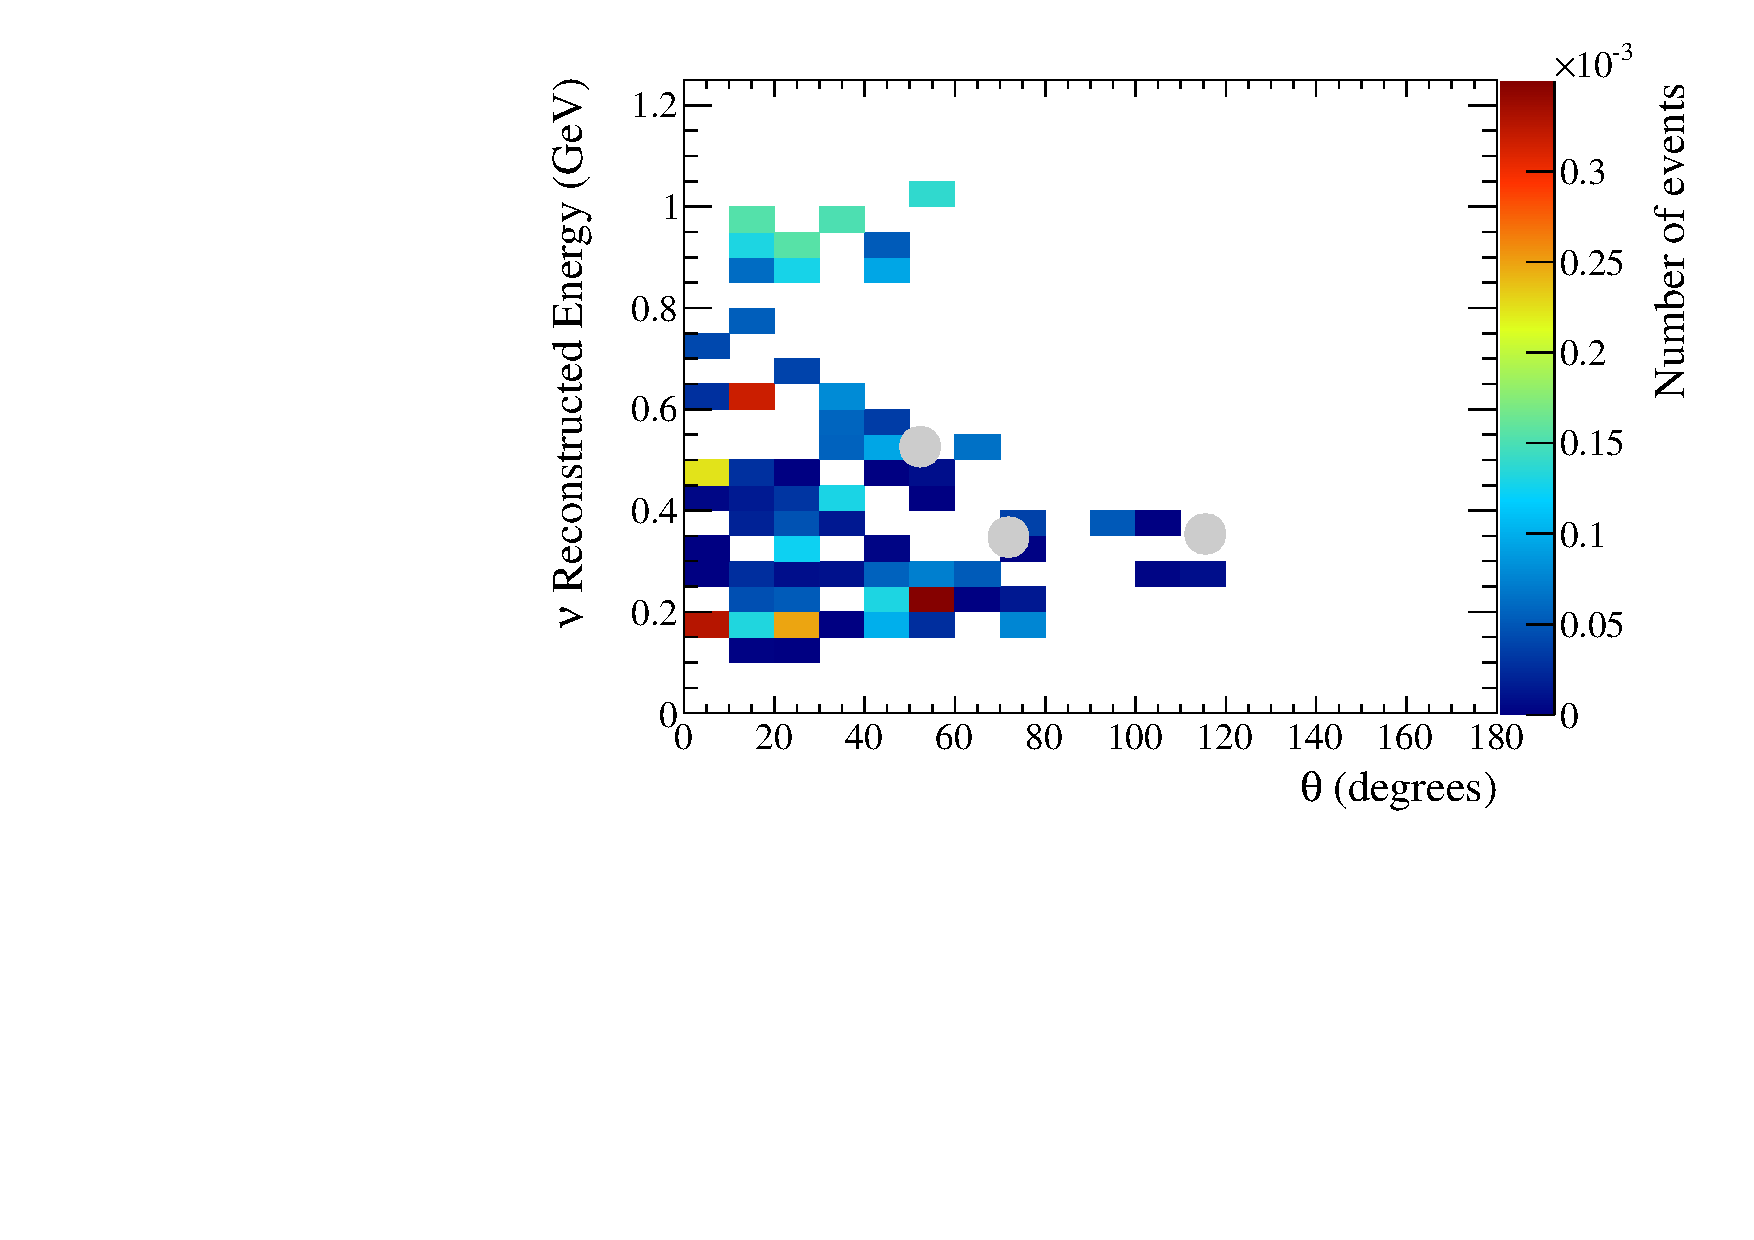
\includegraphics[width=0.9\textwidth]{./joint_plots/data/data_mc_rhc1re_2d_NumuBarBeam.pdf}
\caption{$\bar{\nu}_{\mu}$ intrinsic beam.}
\end{subfigure}
\caption {
Predicted and observed (grey dots) spectra of electron-like events
as a function of the reconstructed neutrino energy and
the angle between the outgoing lepton and the neutrino direction.
The distributions correspond to the collected statistics in the full Run 1-6 data set.
%for an exposure 
%of $6.914 \times 10^{20}$ POT in neutrino  mode.
%and
%of $4.011 \times 10^{20}$ POT in antineutrino mode.
From top left to bottom right the following components are shown:
%total,
$\nu_{\mu} \rightarrow \nu_e$,
$\bar{\nu}_{\mu} \rightarrow \bar{\nu}_e$,
$\nu_e + \bar{\nu}_e$ intrinsic beam,
NC,
$\nu_{\mu}$ intrinsic beam
and
$\bar{\nu}_{\mu}$ intrinsic beam.
The spectra were generated with the systematic parameters measured with the ND280 data 
shown in \cref{tab:banff_uncertainties_flux_fhc},~\ref{tab:banff_uncertainties_flux_rhc},~\ref{tab:banff_uncertainties_xsec},
the nominal Super-K systematic parameters shown in \cref{tab:banff_uncertainties_skdetfsi}
and the oscillation parameters corresponding to the Asimov data set A shown in \cref{tab:osc_params_joint_asimov}.
}
\label{fig:joint_ereco_vs_theta_rhc1re_data}
\end{figure*}


\clearpage


